% Options for packages loaded elsewhere
\PassOptionsToPackage{unicode}{hyperref}
\PassOptionsToPackage{hyphens}{url}
%
\documentclass[
]{report}
\usepackage{amsmath,amssymb}
\usepackage{lmodern}
\usepackage{iftex}
\ifPDFTeX
  \usepackage[T1]{fontenc}
  \usepackage[utf8]{inputenc}
  \usepackage{textcomp} % provide euro and other symbols
\else % if luatex or xetex
  \usepackage{unicode-math}
  \defaultfontfeatures{Scale=MatchLowercase}
  \defaultfontfeatures[\rmfamily]{Ligatures=TeX,Scale=1}
\fi
% Use upquote if available, for straight quotes in verbatim environments
\IfFileExists{upquote.sty}{\usepackage{upquote}}{}
\IfFileExists{microtype.sty}{% use microtype if available
  \usepackage[]{microtype}
  \UseMicrotypeSet[protrusion]{basicmath} % disable protrusion for tt fonts
}{}
\makeatletter
\@ifundefined{KOMAClassName}{% if non-KOMA class
  \IfFileExists{parskip.sty}{%
    \usepackage{parskip}
  }{% else
    \setlength{\parindent}{0pt}
    \setlength{\parskip}{6pt plus 2pt minus 1pt}}
}{% if KOMA class
  \KOMAoptions{parskip=half}}
\makeatother
\usepackage{xcolor}
\usepackage{color}
\usepackage{fancyvrb}
\newcommand{\VerbBar}{|}
\newcommand{\VERB}{\Verb[commandchars=\\\{\}]}
\DefineVerbatimEnvironment{Highlighting}{Verbatim}{commandchars=\\\{\}}
% Add ',fontsize=\small' for more characters per line
\usepackage{framed}
\definecolor{shadecolor}{RGB}{248,248,248}
\newenvironment{Shaded}{\begin{snugshade}}{\end{snugshade}}
\newcommand{\AlertTok}[1]{\textcolor[rgb]{0.94,0.16,0.16}{#1}}
\newcommand{\AnnotationTok}[1]{\textcolor[rgb]{0.56,0.35,0.01}{\textbf{\textit{#1}}}}
\newcommand{\AttributeTok}[1]{\textcolor[rgb]{0.77,0.63,0.00}{#1}}
\newcommand{\BaseNTok}[1]{\textcolor[rgb]{0.00,0.00,0.81}{#1}}
\newcommand{\BuiltInTok}[1]{#1}
\newcommand{\CharTok}[1]{\textcolor[rgb]{0.31,0.60,0.02}{#1}}
\newcommand{\CommentTok}[1]{\textcolor[rgb]{0.56,0.35,0.01}{\textit{#1}}}
\newcommand{\CommentVarTok}[1]{\textcolor[rgb]{0.56,0.35,0.01}{\textbf{\textit{#1}}}}
\newcommand{\ConstantTok}[1]{\textcolor[rgb]{0.00,0.00,0.00}{#1}}
\newcommand{\ControlFlowTok}[1]{\textcolor[rgb]{0.13,0.29,0.53}{\textbf{#1}}}
\newcommand{\DataTypeTok}[1]{\textcolor[rgb]{0.13,0.29,0.53}{#1}}
\newcommand{\DecValTok}[1]{\textcolor[rgb]{0.00,0.00,0.81}{#1}}
\newcommand{\DocumentationTok}[1]{\textcolor[rgb]{0.56,0.35,0.01}{\textbf{\textit{#1}}}}
\newcommand{\ErrorTok}[1]{\textcolor[rgb]{0.64,0.00,0.00}{\textbf{#1}}}
\newcommand{\ExtensionTok}[1]{#1}
\newcommand{\FloatTok}[1]{\textcolor[rgb]{0.00,0.00,0.81}{#1}}
\newcommand{\FunctionTok}[1]{\textcolor[rgb]{0.00,0.00,0.00}{#1}}
\newcommand{\ImportTok}[1]{#1}
\newcommand{\InformationTok}[1]{\textcolor[rgb]{0.56,0.35,0.01}{\textbf{\textit{#1}}}}
\newcommand{\KeywordTok}[1]{\textcolor[rgb]{0.13,0.29,0.53}{\textbf{#1}}}
\newcommand{\NormalTok}[1]{#1}
\newcommand{\OperatorTok}[1]{\textcolor[rgb]{0.81,0.36,0.00}{\textbf{#1}}}
\newcommand{\OtherTok}[1]{\textcolor[rgb]{0.56,0.35,0.01}{#1}}
\newcommand{\PreprocessorTok}[1]{\textcolor[rgb]{0.56,0.35,0.01}{\textit{#1}}}
\newcommand{\RegionMarkerTok}[1]{#1}
\newcommand{\SpecialCharTok}[1]{\textcolor[rgb]{0.00,0.00,0.00}{#1}}
\newcommand{\SpecialStringTok}[1]{\textcolor[rgb]{0.31,0.60,0.02}{#1}}
\newcommand{\StringTok}[1]{\textcolor[rgb]{0.31,0.60,0.02}{#1}}
\newcommand{\VariableTok}[1]{\textcolor[rgb]{0.00,0.00,0.00}{#1}}
\newcommand{\VerbatimStringTok}[1]{\textcolor[rgb]{0.31,0.60,0.02}{#1}}
\newcommand{\WarningTok}[1]{\textcolor[rgb]{0.56,0.35,0.01}{\textbf{\textit{#1}}}}
\usepackage{longtable,booktabs,array}
\usepackage{calc} % for calculating minipage widths
% Correct order of tables after \paragraph or \subparagraph
\usepackage{etoolbox}
\makeatletter
\patchcmd\longtable{\par}{\if@noskipsec\mbox{}\fi\par}{}{}
\makeatother
% Allow footnotes in longtable head/foot
\IfFileExists{footnotehyper.sty}{\usepackage{footnotehyper}}{\usepackage{footnote}}
\makesavenoteenv{longtable}
\usepackage{graphicx}
\makeatletter
\def\maxwidth{\ifdim\Gin@nat@width>\linewidth\linewidth\else\Gin@nat@width\fi}
\def\maxheight{\ifdim\Gin@nat@height>\textheight\textheight\else\Gin@nat@height\fi}
\makeatother
% Scale images if necessary, so that they will not overflow the page
% margins by default, and it is still possible to overwrite the defaults
% using explicit options in \includegraphics[width, height, ...]{}
\setkeys{Gin}{width=\maxwidth,height=\maxheight,keepaspectratio}
% Set default figure placement to htbp
\makeatletter
\def\fps@figure{htbp}
\makeatother
\setlength{\emergencystretch}{3em} % prevent overfull lines
\providecommand{\tightlist}{%
  \setlength{\itemsep}{0pt}\setlength{\parskip}{0pt}}
\setcounter{secnumdepth}{5}
\newlength{\cslhangindent}
\setlength{\cslhangindent}{1.5em}
\newlength{\csllabelwidth}
\setlength{\csllabelwidth}{3em}
\newlength{\cslentryspacingunit} % times entry-spacing
\setlength{\cslentryspacingunit}{\parskip}
\newenvironment{CSLReferences}[2] % #1 hanging-ident, #2 entry spacing
 {% don't indent paragraphs
  \setlength{\parindent}{0pt}
  % turn on hanging indent if param 1 is 1
  \ifodd #1
  \let\oldpar\par
  \def\par{\hangindent=\cslhangindent\oldpar}
  \fi
  % set entry spacing
  \setlength{\parskip}{#2\cslentryspacingunit}
 }%
 {}
\usepackage{calc}
\newcommand{\CSLBlock}[1]{#1\hfill\break}
\newcommand{\CSLLeftMargin}[1]{\parbox[t]{\csllabelwidth}{#1}}
\newcommand{\CSLRightInline}[1]{\parbox[t]{\linewidth - \csllabelwidth}{#1}\break}
\newcommand{\CSLIndent}[1]{\hspace{\cslhangindent}#1}
\usepackage{booktabs}
\usepackage{geometry}
\usepackage[none]{hyphenat}
\usepackage{titlesec}
\usepackage{longtable}
\usepackage{xcolor}
\usepackage{setspace}
\usepackage{pdfpages}

\pagestyle{plain}

%%%% Set margins
\setlength{\topmargin}{-1cm}
\addtolength{\evensidemargin}{-1cm}
\addtolength{\oddsidemargin}{-1cm}
\addtolength{\textheight}{3cm}
\addtolength{\textwidth}{2cm}

% Spacing for reading guides
\newcommand{\rgs}{\vspace{12pt}} % Vertical space
\newcommand{\rgi}{\hspace{24pt}}  % Indent

\newcommand\latexcode[1]{#1}

% Format chapter titles and spacing
\renewcommand*{\chaptername}{Module}

\titleformat{\chapter}[display]
{\bfseries\Large}
{\filleft\MakeUppercase{\chaptertitlename} \Huge\thechapter}
{3ex}
{\titlerule
\vspace{1.5ex}%
\filright}
[\vspace{1.5ex}%
\titlerule]
\titlespacing*{\chapter}{0pt}{-40pt}{20pt}
\ifLuaTeX
  \usepackage{selnolig}  % disable illegal ligatures
\fi
\IfFileExists{bookmark.sty}{\usepackage{bookmark}}{\usepackage{hyperref}}
\IfFileExists{xurl.sty}{\usepackage{xurl}}{} % add URL line breaks if available
\urlstyle{same} % disable monospaced font for URLs
\hypersetup{
  hidelinks,
  pdfcreator={LaTeX via pandoc}}

\title{\textbf{STAT 216 Coursepack}\\
\strut \\
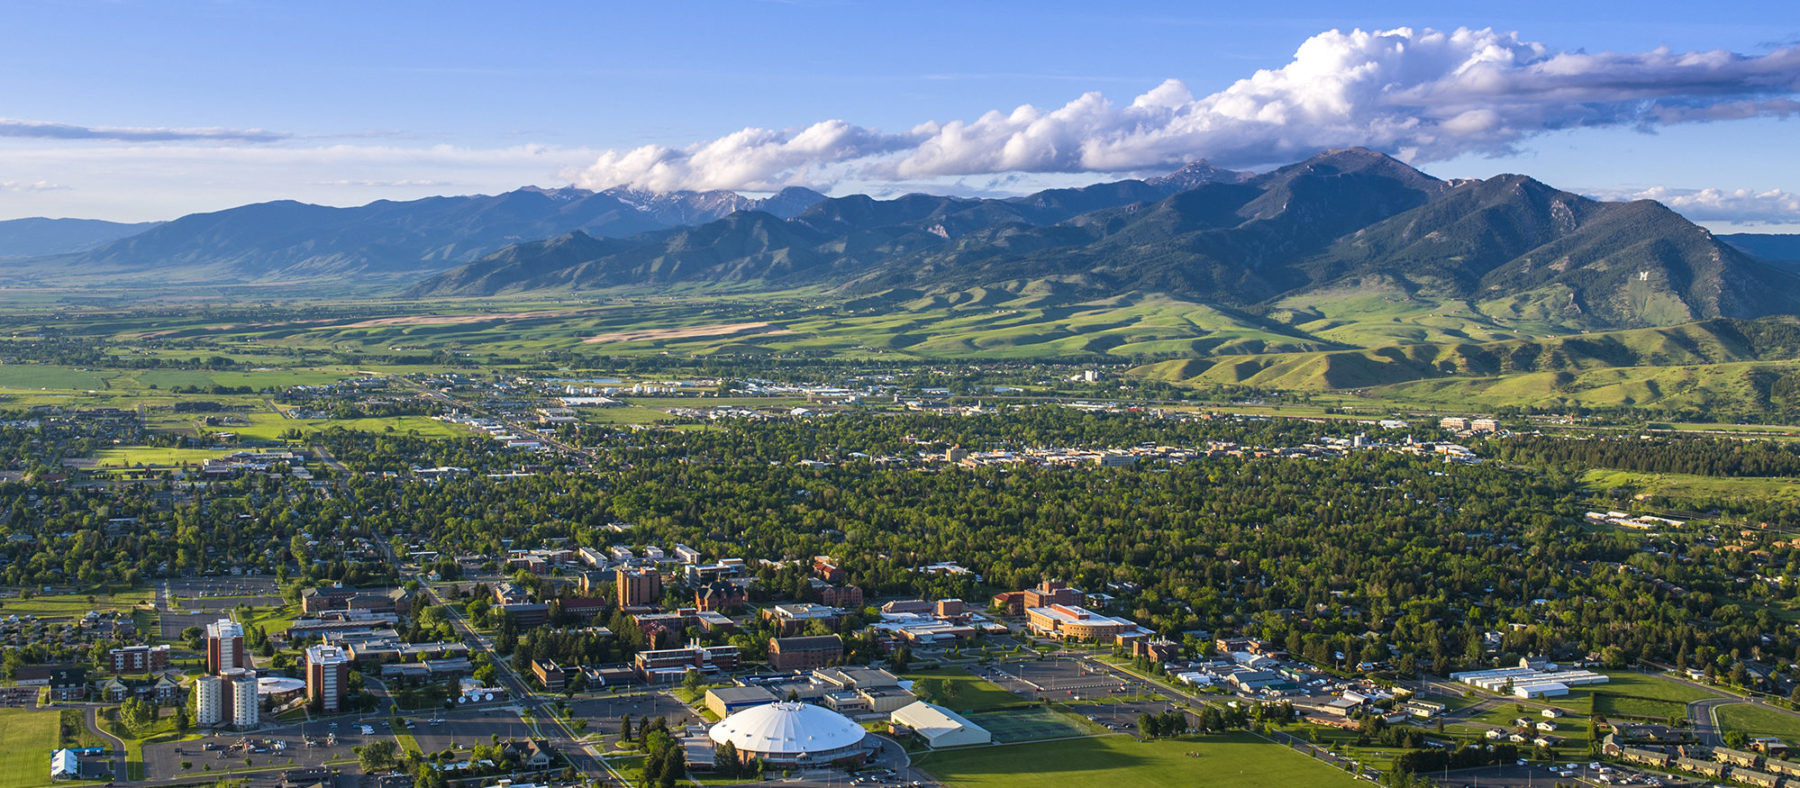
\includegraphics[width=5in,height=\textheight]{images/msu-campus.jpg}}
\usepackage{etoolbox}
\makeatletter
\providecommand{\subtitle}[1]{% add subtitle to \maketitle
  \apptocmd{\@title}{\par {\large #1 \par}}{}{}
}
\makeatother
\subtitle{Fall 2022\\
Montana State University}
\author{Melinda Yager\\
Jade Schmidt\\
Stacey Hancock}
\date{}

\begin{document}
\maketitle

\newpage
\thispagestyle{empty}

This resource was developed by Melinda Yager, Jade Schmidt, and Stacey Hancock in 2021 to accompany the online textbook: Carnegie, N., Hancock, S., Meyer, E., Schmidt, J., and Yager, M. (2021). \emph{Montana State Introductory Statistics with R}. Montana State University. \url{https://mtstateintrostats.github.io/IntroStatTextbook/}.

This resource is released under a \href{https://creativecommons.org/licenses/by-nc-sa/4.0/}{Creative Commons BY-NC-SA 4.0} license unless otherwise noted.

\setcounter{tocdepth}{1}
\addtocontents{toc}{\protect\thispagestyle{empty}}
\tableofcontents
\thispagestyle{empty}

\newpage
\setcounter{page}{1}

\hypertarget{preface}{%
\chapter*{Preface}\label{preface}}
\addcontentsline{toc}{chapter}{Preface}

This coursepack accompanies the textbook for STAT 216: Introduction to Statistics at Montana State University, which can be found at \url{https://mtstateintrostats.github.io/IntroStatTextbook/}. The syllabus for the course (including the course calendar), data sets, and links to D2L Brightspace, Gradescope, and the MSU RStudio server can be found on the course webpage: \url{https://math.montana.edu/courses/s216/}.
Videos assigned in the course calendar and other notes and review materials are linked in D2L.

Each of the activities in this workbook is designed to target specific learning outcomes of the course, giving you practice with important statistical concepts in a group setting with instructor guidance. In addition to the in-class activities for the course, the coursepack includes reading guides to aid in taking notes while you complete the required readings and videos. Bring this workbook with you to class each class period, and take notes in the workbook as you would your own notes. A well-written completed workbook will provide an optimal study guide for exams!

The activities and labs in this coursepack will be completed during class time. Parts of each lab will be turned in on Gradescope. To aid in your understanding, read through the introduction for each activity before attending class each day.

STAT 216 is a 3-credit in-person course. In our experience, it takes six to nine hours per week outside of class to achieve a good grade in this class. By ``good'' we mean at least a C because a grade of D or below does not count toward fulfilling degree requirements. Many of you set your goals higher than just getting a C, and we fully support that. You need roughly nine hours per week to review past activities, read feedback on previous assignments, complete current assignments, and prepare for the next day's class. A typical week in the life of a STAT 216 student looks like:

\begin{itemize}
\tightlist
\item
  \emph{Prior to class meeting}:

  \begin{itemize}
  \tightlist
  \item
    Read assigned sections of the textbook, using the provided reading guides to take notes on the material.
  \item
    Watch assigned videos on that week's content, pausing to take notes and answer video quiz questions.
  \item
    Read through the introduction to the day's in-class activity
  \item
    Read through the week's homework assignment and note any questions you may have on the content.
  \end{itemize}
\item
  \emph{During class meeting}:

  \begin{itemize}
  \tightlist
  \item
    Work through the in-class activity or weekly lab with your classmates and instructor, taking detailed notes on your answers to each question in the activity.
  \end{itemize}
\item
  \emph{After class meeting}:

  \begin{itemize}
  \tightlist
  \item
    Complete any parts of the activity you did not complete in class.
  \item
    Review the activity solutions in the Math and Stat Center, and take notes on key points.
  \item
    Finish watching any remaining assigned videos or readings for the week.
  \item
    Complete the week's homework assignment.
  \end{itemize}
\end{itemize}

\nocite{*}

\hypertarget{activity-1-intro-to-data}{%
\section{Activity 1: Intro to Data}\label{activity-1-intro-to-data}}

\setstretch{1}

\hypertarget{learning-outcomes}{%
\subsection{Learning outcomes}\label{learning-outcomes}}

\begin{itemize}
\item
  Identify observational units, variables, and variable types in a statistical study.
\item
  Identify biased sampling methods.
\end{itemize}

\hypertarget{terminology-review}{%
\subsection{Terminology review}\label{terminology-review}}

Statistics is the study of how best to collect, analyze, and draw conclusions from data. Today in class you will be introduced to the following terms:

\begin{itemize}
\item
  Observational units or cases
\item
  Variables: categorical or quantitative
\item
  Types of sampling bias
\end{itemize}

For more on these concepts, read Chapter 1 and Section 2.1 in the textbook.

\hypertarget{general-information-on-labs}{%
\subsection{General information on labs}\label{general-information-on-labs}}

On Friday of each week you will complete a lab. Questions are selected from each lab to be turned in on Gradescope. The questions to be submitted on Gradescope are bolded in the lab. As you work through the lab have the Gradescope lab assignment open so that you can answer those questions as you go. Today's activity is Lab 0 in Gradescope for practice submitting as a group.

\hypertarget{steps-of-the-statistical-investigation-process}{%
\subsubsection*{Steps of the statistical investigation process}\label{steps-of-the-statistical-investigation-process}}
\addcontentsline{toc}{subsubsection}{Steps of the statistical investigation process}

As we move through the semester we will work through the six steps of the statistical investigation process.

\begin{enumerate}
\def\labelenumi{\arabic{enumi}.}
\item
  Ask a research question.
\item
  Design a study and collect data.
\item
  Summarize and visualize the data. \emph{Weeks 3--4}
\item
  Use statistical analysis methods to draw inferences from the data. \emph{Weeks 6--13}
\item
  Communicate the results and answer the research question. \emph{Weeks 6--13}
\item
  Revisit and look forward.
\end{enumerate}

Today we will focus on the first two steps.

\textbf{Step 1}: The first step of any statistical investigation is to \emph{ask a research question}. As stated in the textbook, ``with the rise of data science, however, we might not start with a research question, and instead start with a data set.'' Today we will create a data set by collecting responses on students in class.

\textbf{Step 2}: To answer any research question, we must \emph{design a study and collect data}. Our study will consist of answers from each student. Your responses will become our observed data that we will explore.

\textbf{Observational units} or \textbf{cases} are the subjects data are collected on. In a spreadsheet of the data set, each row will represent a single observational unit.

\begin{enumerate}
\def\labelenumi{\arabic{enumi}.}
\tightlist
\item
  \textbf{What are the observational units or cases for today's study? }
\end{enumerate}

\vspace{0.2in}

\begin{enumerate}
\def\labelenumi{\arabic{enumi}.}
\setcounter{enumi}{1}
\tightlist
\item
  How many students are in class today? This is the \textbf{sample size}.
\end{enumerate}

\vspace{0.2in}

A \textbf{variable} is information collected or measured on each observational unit or case. Each column in a data set will represent a different variable.

One person from each group at each table, open the Google sheet linked in D2L and fill in the responses for the following questions for each group member. When creating a data set for use in R it is important to use single words or an underscore between words. Each outcome must be written the same way each time. Make sure to use all lowercase letters to create this data set to have consistency between responses. Do not give units of measure with the numerical values for the length of forearm. For \texttt{Residency} use in\_state or out\_state as the two outcomes.

\begin{itemize}
\tightlist
\item
  Major: what is your declared major?
\item
  Residency: do you have in-state or out-of-state residency?
\item
  Forearm\_Length: what is the length of your forearm in inches from the end of your elbow to the end of your index finger?
\item
  Num\_Credits: how many credits are you taking this semester?
\end{itemize}

We will look at two types of variables: \textbf{quantitative} and \textbf{categorical} (see Figure \ref{fig:types-of-variables}).

Quantitative variables are numerical measurements that can be discrete (whole, non-negative numbers) or continuous (any value within an interval). The number of pets one owns would be a discrete variable as you can not have a partial pet. GPA would be a continuous variable ranging from 0 to 4.0.

The outcome of a categorical variable is a group or category such as eye color, state of residency, or whether or not a student lives on campus. Categorical variables with a natural ordering are considered ordinal variables while those without a natural ordering are considered nominal variables. All categorical variables will be treated as nominal for analysis in this course.

\begin{figure}

{\centering 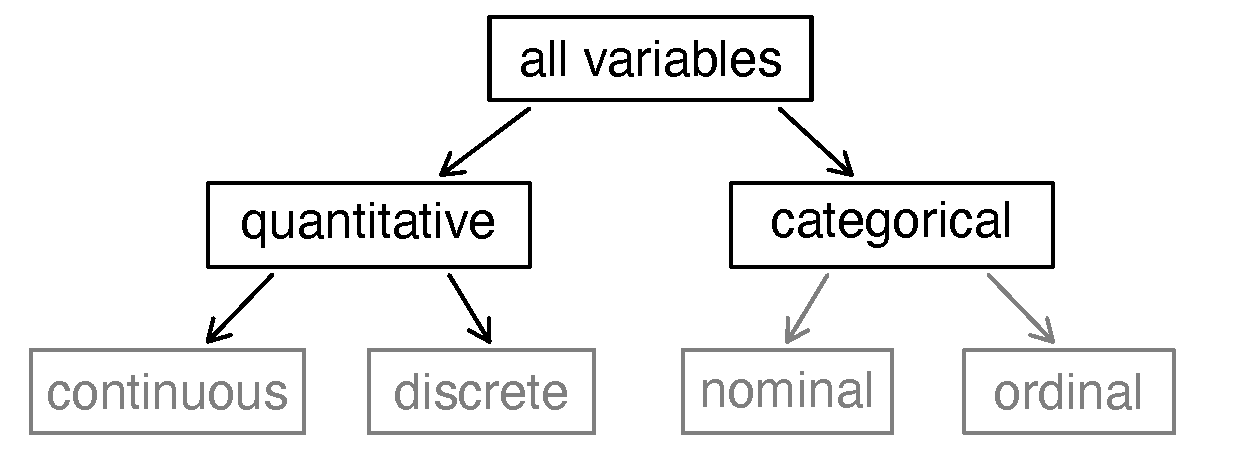
\includegraphics[width=0.5\linewidth]{images/variables} 

}

\caption{Types of variables.}\label{fig:types-of-variables}
\end{figure}

\newpage

\begin{enumerate}
\def\labelenumi{\arabic{enumi}.}
\setcounter{enumi}{2}
\tightlist
\item
  For each column of data, fill in the following table to write out the variable we are collecting on each observational unit in this study and the type of each variable.
\end{enumerate}

\begin{center}
\begin{tabular}{|l|p{2in}|p{2in}|} \hline
Column & Variable & Type of Variable  \\ \hline
Major & & \\ 
& & \\ \hline
Residency & & \\ 
& & \\ \hline
Forearm Length & & \\ 
& & \\ \hline
Num Credits & & \\ 
& & \\ \hline
\end{tabular}
\end{center}

In the next few weeks we will look at how to summarize data both numerically and graphically. For now we will focus on sampling methods and the type of sampling bias that may be present.

\begin{itemize}
\item
  Sampling bias: a part of the target population is not included or underrepresented in the sample
\item
  Non-response or non-participation bias: part of the already selected population does not respond or chooses not to participate
\item
  Response bias: survey participant gives an untruthful or misleading response
\end{itemize}

To help determine the type of bias present, it is helpful to think about the observational units, the sample and the target population represented by the problem. The \textbf{target population} is the group of cases that makes up the population the researcher is interested in. If sampling bias is present, than the sample taken will not be representative of the actual target population. In these next questions, identify the target population, the sample selected, the variable collected and its type (categorical or quantitative), and the type of bias present.

\begin{enumerate}
\def\labelenumi{\arabic{enumi}.}
\setcounter{enumi}{3}
\item
  \textbf{To determine if the proportion of out-of-state undergraduate students at Montana State University has increased in the last 10 years, a statistics instructor sent an email survey to 500 randomly selected current undergraduate students. One of the questions on the survey asked whether they had in-state or out-of-state residency. She only received 378 responses.}
  \vspace{0.25in}

  Observational units or cases:
  \vspace{0.3in}

  Target population:
  \vspace{0.3in}

  Sample size:
  \vspace{0.3in}

  Sample taken:
  \vspace{0.3in}

  Variable:
  \vspace{0.3in}

  Type of Variable: \hspace{1mm} categorical \hspace{0.2in} quantitative
  \vspace{1mm}

  Type(s) of bias:
  \vspace{0.3in}
\item
  A television station is interested in predicting whether or not a local referendum to legalize marijuana for adult use will pass. It asks its viewers to phone in and indicate whether they are in favor or opposed to the referendum. Of the 2241 viewers who phoned in, forty-five percent were opposed to legalizing marijuana.
  \vspace{0.1in}

  Observational units or cases:
  \vspace{0.3in}

  Target population:
  \vspace{0.3in}

  Sample size:
  \vspace{0.3in}

  Sample taken:
  \vspace{0.3in}

  Variable:
  \vspace{0.3in}

  Type of Variable: \hspace{1mm} categorical \hspace{0.2in} quantitative
  \vspace{1mm}

  Type(s) of bias:
  \vspace{0.3in}
\item
  To gauge the interest in a new swimming pool, a local organization stood outside of the Bogart Pool in Bozeman, MT, during open hours. One of the questions they asked was, ``Since the Bogart Pool is in such bad repair, don't you agree that the city should fund a new pool?''
  \vspace{0.1in}

  Observational units or cases:
  \vspace{0.3in}

  Target population:
  \vspace{0.3in}

  Sample size:
  \vspace{0.3in}

  Sample taken:
  \vspace{0.3in}

  Variable:
  \vspace{0.3in}

  Type of Variable: \hspace{1mm} categorical \hspace{0.2in} quantitative
  \vspace{1mm}

  Type(s) of bias:
  \vspace{0.3in}
\end{enumerate}

\newpage

\begin{enumerate}
\def\labelenumi{\arabic{enumi}.}
\setcounter{enumi}{6}
\tightlist
\item
  \textbf{The Bozeman school district was interested in surveying parents of students about their opinions on returning to in-person classes following the COVID-19 pandemic. They divided the school district into 10 divisions based on location and randomly surveyed 20 households within each division. Explain why selection bias would be present in this study design.}
  \vspace{1in}
\end{enumerate}

\hypertarget{take-home-messages}{%
\subsection{Take-home messages}\label{take-home-messages}}

\begin{enumerate}
\def\labelenumi{\arabic{enumi}.}
\item
  When creating a data set, each row will represent a single observational unit or case. Each column represents a variable collected. It is important to write each variable as a single word or use an underscore between words.
\item
  There are two types of variables: categorical (groups) and quantitative (numerical measures).
\item
  There are three types of bias to be aware of when designing a sampling method: selection bias, non-response bias, and response bias.
\end{enumerate}

\hypertarget{additional-notes}{%
\subsection{Additional notes}\label{additional-notes}}

Use this space to summarize your thoughts and take additional notes on today's activity and material covered, and to write down the names and contact information of your teammates.

\newpage

\hypertarget{out-of-class-activity-2-american-indian-address}{%
\section{OUt of Class Activity 2: American Indian Address}\label{out-of-class-activity-2-american-indian-address}}

\setstretch{1}

\hypertarget{learning-outcomes-1}{%
\subsection{Learning outcomes}\label{learning-outcomes-1}}

\begin{itemize}
\item
  Explain why a sampling method is unbiased or biased.
\item
  Identify biased sampling methods.
\item
  Explain the purpose of random selection and its effect on scope of inference.
\end{itemize}

\hypertarget{terminology-review-1}{%
\subsection{Terminology review}\label{terminology-review-1}}

In this activity, we will examine unbiased and biased methods of sampling. Some terms covered in this activity are:

\begin{itemize}
\item
  Random sample
\item
  Unbiased vs biased methods of selection
\item
  Generalization
\end{itemize}

To review these concepts, see Section 1.3 in the textbook.

\hypertarget{american-indian-address}{%
\subsection{American Indian Address}\label{american-indian-address}}

Complete questions 1 - 4 in class. Your instructor will create and post the distribution needed for the remainder of the activity by 8 pm on Monday night. For this activity, you will read a speech given by Jim Becenti, a member of the Navajo American Indian tribe, who spoke about the employment problems his people faced at an Office of Indian Affairs meeting in Phoenix, Arizona, on January 30, 1947 (Moquin and Van Doren 1973). His speech is below:

\textbf{It is hard for us to go outside the reservation where we meet strangers. I have been off the reservation ever since I was sixteen. Today I am sorry I quit the Santa Fe {[}Railroad{]}. I worked for them in 1912-13. You are enjoying life, liberty, and happiness on the soil the American Indian had, so it is your responsibility to give us a hand, brother. Take us out of distress. I have never been to vocational school. I have very little education. I look at the white man who is a skilled laborer. When I was a young man I worked for a man in Gallup as a carpenter's helper. He treated me as his own brother. I used his tools. Then he took his tools and gave me a list of tools I should buy and I started carpentering just from what I had seen. We have no alphabetical language.}

\textbf{We see things with our eyes and can always remember it. I urge that we help my people to progress in skilled labor as well as common labor. The hope of my people is to change our ways and means in certain directions, so they can help you someday as taxpayers. If not, as you are going now, you will be burdened the rest of your life. The hope of my people is that you will continue to help so that we will be all over the United States and have a hand with you, and give us a brotherly hand so we will be happy as you are. Our reservation is awful small. We did not know the capacity of the range until the white man come and say ``you raise too much sheep, got to go somewhere else,'' resulting in reduction to a skeleton where the Indians can't make a living on it. For eighty years we have been confused by the general public, and what is the condition of the Navajo today? Starvation! We are starving for education. Education is the main thing and the only thing that is going to make us able to compete with you great men here talking to us.}

\hypertarget{by-eye-selection}{%
\subsubsection*{By eye selection}\label{by-eye-selection}}
\addcontentsline{toc}{subsubsection}{By eye selection}

\begin{enumerate}
\def\labelenumi{\arabic{enumi}.}
\tightlist
\item
  Circle ten words in Jim Becenti's speech which are a representative sample of the length of words in the entire text. Describe your method for selecting this sample.
\end{enumerate}

\vspace{0.3in}

\begin{enumerate}
\def\labelenumi{\arabic{enumi}.}
\setcounter{enumi}{1}
\tightlist
\item
  Fill in the table below with your selected words from the previous question and the length of each word (number of letters/digits in the word):
  \vspace{1mm}
\end{enumerate}

\begin{center}
\begin{tabular}{|l|p{3in}|p{1in}|} \hline
Observation & Word & Length  \\ \hline
1 & & \\ 
& & \\ \hline
2 & & \\ 
& & \\ \hline
3 & & \\ 
& & \\ \hline
4 & & \\ 
& & \\ \hline
5 & & \\ 
& & \\ \hline
6 & & \\ 
& & \\ \hline
7 & & \\
& & \\ \hline
8 & & \\ 
& & \\ \hline
9 & & \\ 
& & \\ \hline
10 & & \\ 
& & \\ \hline
\end{tabular}
\end{center}

\begin{enumerate}
\def\labelenumi{\arabic{enumi}.}
\setcounter{enumi}{2}
\item
  Calculate the mean (average) word length in your selected sample. Is this value a parameter or a statistic?\\
  \vspace{0.3in}
\item
  Report your mean word length in the google spreadsheet. Your instructor will create a visualization of the distribution of results generated by your class. Draw a picture of the plot here. Include a descriptive \(x\)-axis label.
  \vspace{1.5in}
\item
  Based on the plot of sample mean word lengths in question 4, what is your best guess for the average word length of the population of all 359 words in the speech?
  \vspace{0.3in}
\item
  The true mean word length of the population of all 359 words in the speech is 3.95 letters. Is this value a parameter or a statistic?\\
  \vspace{0.2in}

  Where does the value of 3.95 fall in the plot created in question 4? Near the center of the distribution? In the tails of the distribution?
  \vspace{0.3in}
\item
  If the class samples were truly representative of the population of words, what proportion of sample means would you expect to be below 3.95?
  \vspace{0.5in}
\item
  Using the graph created in question 4, estimate the proportion of students' computed sample means that were lower than the true mean of 3.95 letters?
  \vspace{0.5in}
\item
  Based on your answers to questions 7 and 8, would you say the sampling method used by the class is biased or unbiased? Justify your answer.\\
  \vspace{0.5in}
\item
  If the sampling method is biased, what type of sampling bias (selection, response, non-response) is present? What is the direction of the bias, i.e., does the method tend to overestimate or underestimate the population mean word length?
  \vspace{0.5in}
\item
  Should we use results from our by eye samples to make a statement about the word length in the population of words in Becenti's address? Why or why not?
  \vspace{1in}
\end{enumerate}

\hypertarget{take-home-messages-1}{%
\subsection{Take-home messages}\label{take-home-messages-1}}

\begin{enumerate}
\def\labelenumi{\arabic{enumi}.}
\item
  When we use a biased method of selection, we will over or underestimate the parameter.
\item
  To see if a method is biased, we compare the distribution of the estimates to the true value. We want our estimate to be on target or unbiased. When using unbiased methods of selection, the mean of the distribution matches or is very similar to our true parameter.
\item
  If the sampling method is biased, inferences made about the population based on a sample estimate will not be valid.
\end{enumerate}

\hypertarget{additional-notes-1}{%
\subsection{Additional notes}\label{additional-notes-1}}

Use this space to summarize your thoughts and take additional notes on today's activity and material covered.

\newpage

\hypertarget{activity-2-american-indian-address-continued}{%
\section{Activity 2: American Indian Address (continued)}\label{activity-2-american-indian-address-continued}}

\setstretch{1}

\hypertarget{learning-outcomes-2}{%
\subsection{Learning outcomes}\label{learning-outcomes-2}}

\begin{itemize}
\item
  Explain the purpose of random selection and its effect on scope of inference.
\item
  Select a simple random sample from a finite population using a random number generator.
\item
  Explain why a sampling method is unbiased or biased.
\item
  Explain the effect of sample size on sampling variability.
\end{itemize}

\hypertarget{terminology-review-2}{%
\subsection{Terminology review}\label{terminology-review-2}}

In today's activity, we will examine unbiased and biased methods of sampling. Some terms covered in this activity are:

\begin{itemize}
\item
  Random sample
\item
  Unbiased vs biased methods of selection
\item
  Generalization
\end{itemize}

To review these concepts, see Section 2.1 in the textbook.

\hypertarget{random-selection}{%
\subsubsection*{Random selection}\label{random-selection}}
\addcontentsline{toc}{subsubsection}{Random selection}

Today we will return to the American Indian Address introduced in the out of class activity. Suppose instead of attempting to select a representative sample by eye (which did not work), each student used a random number generator to select a simple random sample of 10 words. A \textbf{simple random sample} relies on a random mechanism to choose a sample, without replacement, from the population, such that every sample of size 10 is equally likely to be chosen.

To use a random number generator to select a simple random sample, you first need a numbered list of all the words in the population, called a \textbf{sampling frame}. You can then generate 10 random numbers from the numbers 1 to 359 (the number of words in the population), and the chosen random numbers correspond to the chosen words in your sample.

\begin{enumerate}
\def\labelenumi{\arabic{enumi}.}
\tightlist
\item
  Use the random number generator at \url{https://istats.shinyapps.io/RandomNumbers/} to select a simple random sample from the population of all 359 words in the speech.
\end{enumerate}

\begin{itemize}
\item
  Set ``Choose Minimum'' to 1 and ``Choose Maximum'' to 359 to represent the 359 words in the population (the sampling frame).
\item
  Set ``How many numbers do you want to generate?'' to 10 and ensure the ``No'' option is selected under ``Sample with Replacement?''
\item
  Click ``Generate''.
\end{itemize}

\newpage

Fill in the table below with the random numbers selected and use the Becenti.csv data file found on D2L to determine each number's corresponding word and word length (number of letters/digits in the word):

\begin{center}
\begin{tabular}{|l|l|p{3in}|p{1in}|} \hline
Observation & Number & Word & Length  \\ \hline
1 & & & \\ 
& & & \\ \hline
2 & & & \\ 
& & & \\ \hline
3 & & & \\ 
& & & \\ \hline
4 & & & \\ 
& & & \\ \hline
5 & & & \\ 
& & & \\ \hline
6 & & & \\ 
& & & \\ \hline
7 & & & \\
& & & \\ \hline
8 & & & \\ 
& & & \\ \hline
9 & & &\\ 
& & & \\ \hline
10 & & & \\ 
& & & \\ \hline
\end{tabular}
\end{center}

``

\begin{enumerate}
\def\labelenumi{\arabic{enumi}.}
\setcounter{enumi}{1}
\item
  Calculate the mean word length in your selected sample in question 1. Is this value a parameter or a statistic?
  \vspace{0.3in}
\item
  Report your mean word length to your instructor. Your instructor will guide the class in creating a visualization of the distribution of results generated by your class. Draw a picture of the plot here. Include a descriptive \(x\)-axis label.
  \vspace{1.7in}
\item
  Where does the value 3.95, the true mean word length, fall in the distribution created in question 3? Near the center of the distribution? In the tails of the distribution?
  \vspace{0.3in}
\end{enumerate}

\newpage

\begin{enumerate}
\def\labelenumi{\arabic{enumi}.}
\setcounter{enumi}{4}
\tightlist
\item
  How does the plot generated in question 3 compare to the plot generated in question 4 from Activity 2A?
\end{enumerate}

\rgi Which features are similar?\\
\vspace{0.4in}

\rgi Which features differ?

\vspace{0.4in}

\rgi Why didn't everyone get the same sample mean?
\vspace{0.4in}

One set of randomly generated sample mean word lengths from a single class may not be large enough to visualize the distribution results. Let's have a computer generate 1,000 sample mean word lengths for us.

\begin{itemize}
\item
  Navigate to the ``One Variable with Sampling'' Rossman/Chance web applet: \url{http://www.rossmanchance.com/applets/2021/sampling/OneSample.html?population=gettysburg}.
\item
  Click ``Clear'' below the text box containing data from the Gettysburg address to delete that data set.
\item
  Download the Becenti.csv file from D2L and open the spreadsheet on your computer.
\item
  Copy and paste the population of word lengths (column C) into the applet from the data set provided making sure to include the header. Click ``Use Data''. Verify that the mean for the data set is 3.953 with a sample size of 359. If these are not the values you got, check with your instructor for help with copying in the data set correctly.
\item
  Click the check-box for ``Show Sampling Options''
\item
  Select 1000 for ``Number of samples'' and select 10 for the ``Sample size''.
\item
  Click ``Draw Samples''.
\end{itemize}

\begin{enumerate}
\def\labelenumi{\arabic{enumi}.}
\setcounter{enumi}{5}
\item
  The plot labeled ``Statistics'' displays the 1,000 randomly generated sample mean word lengths. Sketch this plot below. Include a descriptive \(x\)-axis label and be sure to write down the provided mean and SD (standard deviation) of the distribution.
  \vspace{1.5in}
\item
  What is the center value of the distribution created in question 6?
  \vspace{0.3in}
\end{enumerate}

\newpage

\begin{enumerate}
\def\labelenumi{\arabic{enumi}.}
\setcounter{enumi}{7}
\item
  Explain why the sampling method of using a random number generator to generate a sample is a ``better'' method than choosing 10 words ``by eye''.
  \vspace{0.8in}
\item
  Is random selection an unbiased method of selection? Explain your answer. Be sure to reference your plot from question 6.
  \vspace{0.5in}
\end{enumerate}

\hypertarget{effect-of-sample-size}{%
\subsection*{Effect of sample size}\label{effect-of-sample-size}}
\addcontentsline{toc}{subsection}{Effect of sample size}

We will now consider the impact of sample size.

\begin{enumerate}
\def\labelenumi{\arabic{enumi}.}
\setcounter{enumi}{9}
\item
  First, consider if each student had selected 20 words, instead of 10, by eye. Do you think this would make the plot from question 4 in Activity 2A centered on 3.95 (the true mean word length)? Explain your answer.
  \vspace{0.4in}
\item
  Now we will select 20 words instead of 10 words at random.
\end{enumerate}

\begin{itemize}
\item
  In the ``One Variable with Sampling'' Rossman/Chance web applet(\url{http://www.rossmanchance.com/applets/2021/sampling/OneSample.html?population=gettysburg}.), change the Sample size to 20.
\item
  Click ``Draw Samples''.
\end{itemize}

The plot labeled ``Statistics'' displays the 1,000 randomly generated sample mean word lengths. Sketch this plot below. Include a descriptive \(x\)-axis label and be sure to write down the provided mean and SD (standard deviation) of the distribution.
\vspace{1.6in}

\begin{enumerate}
\def\labelenumi{\arabic{enumi}.}
\setcounter{enumi}{11}
\tightlist
\item
  Compare the distribution created in question 11 to the one created in question 6.
\end{enumerate}

\rgi Which features are similar?\\
\vspace{0.3in}

\rgi Which features differ?

\vspace{0.3in}

\newpage

\begin{enumerate}
\def\labelenumi{\arabic{enumi}.}
\setcounter{enumi}{12}
\item
  Compare the spreads of the plots in question 11 and in question 6. You should see that in one plot all sample means are closer to the population mean than in the other. Which plot shows this?
  \vspace{0.4in}
\item
  Using the evidence from your simulations, answer the following research questions:
\end{enumerate}

\rgi Does changing the sample size impact whether the sample estimates are unbiased? Explain your answer.
\vspace{0.5in}

\rgi Does changing the sample size impact the variability (spread) of sample estimates? Explain your answer
\vspace{0.5in}

\begin{enumerate}
\def\labelenumi{\arabic{enumi}.}
\setcounter{enumi}{14}
\tightlist
\item
  What is the purpose of random selection of a sample from the population?
\end{enumerate}

\vspace{0.8in}

\hypertarget{take-home-messages-2}{%
\subsection{Take-home messages}\label{take-home-messages-2}}

\begin{enumerate}
\def\labelenumi{\arabic{enumi}.}
\item
  Random selection is an unbiased method of selection.
\item
  To determine if a sampling method is biased or unbiased, we compare the distribution of the estimates to the true value. We want our estimate to be on target or unbiased. When using unbiased methods of selection, the mean of the distribution matches or is very similar to our true parameter.
\item
  Random selection eliminates selection bias. However, random selection will not eliminate response or non-response bias.
\item
  The larger the sample size, the more similar (less variable) the statistics will be from different samples.
\item
  Sample size has no impact on whether a \emph{sampling method} is biased or not. Taking a larger sample using a biased method will still result in a sample that is not representative of the population.
\end{enumerate}

\hypertarget{additional-notes-2}{%
\subsection{Additional notes}\label{additional-notes-2}}

Use this space to summarize your thoughts and take additional notes on today's activity and material covered.

\newpage

\hypertarget{week-2-lab-study-design}{%
\section{Week 2 Lab: Study Design}\label{week-2-lab-study-design}}

\setstretch{1}

\hypertarget{learning-outcomes-3}{%
\subsection{Learning outcomes}\label{learning-outcomes-3}}

\begin{itemize}
\item
  Explain the purpose of random assignment and its effect on scope of inference.
\item
  Identify whether a study design is observational or an experiment.
\item
  Identify confounding variables in observational studies and explain why they are confounding.
\end{itemize}

\hypertarget{terminology-review-3}{%
\subsection{Terminology review}\label{terminology-review-3}}

In this activity, we will examine different study designs, confounding variables, and how to determine the scope of inference for a study. Some terms covered in this activity are:

\begin{itemize}
\item
  Scope of inference
\item
  Explanatory variable
\item
  Response variable
\item
  Confounding variable
\item
  Experiment
\item
  Observational study
\end{itemize}

To review these concepts, see Sections 2.2 through 2.5 in the textbook.

\hypertarget{general-information-labs}{%
\subsection{General information labs}\label{general-information-labs}}

Remember that each Friday you will complete a lab. Questions are selected from each lab to be turned in on Gradescope. The questions to be submitted on Gradescope are bolded in the lab. As you work through the lab have the Gradescope lab assignment open so that you can answer those questions as you go.

\hypertarget{study-design}{%
\subsection*{Study design}\label{study-design}}
\addcontentsline{toc}{subsection}{Study design}

The two main study designs we will cover are \textbf{observational studies} and \textbf{experiments}. In observational studies, researchers have no influence over which subjects are in each group being compared (though they can control other variables in the study). An experiment is defined by assignment of the treatment groups of the \emph{explanatory variable}, typically via random assignment. In today's activity we will discover the purpose behind random assignment.

For the next exercises, identify the explanatory variable, the response variable, and the study design (observational study or experiment).

\newpage

\begin{enumerate}
\def\labelenumi{\arabic{enumi}.}
\item
  The pharmaceutical company Moderna Therapeutics, working in conjunction with the National Institutes of Health, conducted Phase 3 clinical trials of a vaccine for COVID-19 last fall. US clinical research sites enrolled 30,000 volunteers without COVID-19 to participate. Participants were randomly assigned to receive either the candidate vaccine or a saline placebo. They were then followed to assess whether or not they developed COVID-19. The trial was double-blind, so neither the investigators nor the participants knew who was assigned to which group.
  \vspace{0.1in}

  Explanatory variable:
  \vspace{0.25in}

  Response variable:
  \vspace{0.25in}

  Study design:
  \vspace{0.25in}
\item
  \textbf{In another study, a local health department randomly selected 1000 US adults without COVID-19 to participate in a health survey. Each participant was assessed at the beginning of the study and then followed for one year. They were interested to see which participants elected to receive a vaccination for COVID-19 and whether any participants developed COVID-19.}
  \vspace{0.1in}

  Explanatory variable:
  \vspace{0.25in}

  Response variable:
  \vspace{0.25in}

  Study design:
  \vspace{0.25in}
\end{enumerate}

\hypertarget{atrial-fibrillation}{%
\subsection*{Atrial fibrillation}\label{atrial-fibrillation}}
\addcontentsline{toc}{subsection}{Atrial fibrillation}

Atrial fibrillation is an irregular and often elevated heart rate. In some people, atrial fibrillation will come and go on its own, but others will experience this condition on a permanent basis. When atrial fibrillation is constant, medications are required to stabilize the patient's heart rate and to help prevent blood clots from forming. Pharmaceutical scientists at a large pharmaceutical company believe they have developed a new medication that effectively stabilizes heart rates in people with permanent atrial fibrillation. They set out to conduct a trial study to investigate the new drug. The scientists will need to compare the proportion of patients whose heart rate is stabilized between two groups of subjects, one of whom is given a placebo and the other given the new medication.

\begin{enumerate}
\def\labelenumi{\arabic{enumi}.}
\setcounter{enumi}{2}
\item
  Identify the explanatory and response variable in this trial study.

  Explanatory variable:
  \vspace{0.5in}

  Response variable:
  \vspace{0.5in}
\end{enumerate}

\newpage

Suppose 24 subjects with permanent atrial fibrillation have volunteered to participate in this study:

Self-identified males: Paul, Antonio, Davieon, Chao, Aryan, Jabari, Tong, Andres, John, Liu, Lucas, Rashidi, Shiwoo, Jihoon, Alejandro, Daniel

Self-identified females: An, Nailah, Jasmine, Ka Nong, Keyaina, Mary, Adah, Sassandra

\begin{enumerate}
\def\labelenumi{\arabic{enumi}.}
\setcounter{enumi}{3}
\item
  Is this a simple random sample or a convenience sample? How do you know?
  \vspace{0.5in}
\item
  Based on the sampling method, to what population should the results of this study be generalized?
  \vspace{0.5in}
\item
  One way to separate into two groups would be give all the males the placebo and all the females the new drug. Would this be a reasonable strategy? Explain your answer.
  \vspace{1in}
\item
  Could the scientists fix the problem with the strategy presented in question 6 by creating equal sized groups by putting 4 males and 8 females into the drug group and the remaining 12 males in the placebo group? Explain your answer.
  \vspace{0.5in}
\item
  A third strategy would be to \textbf{block} on sex. In this type of study, the scientists would assign 4 females and 8 males to each group. Using this strategy, what proportion of males is in each group?
  \vspace{0.3in}
\item
  \textbf{Assume the scientists used the strategy in question 8, but they put the four tallest females and eight tallest males into the placebo group and the remaining subjects into the control group. They found that the proportion of patients whose heart rate stabilized is higher in the drug group than the placebo group.}\\
  \vspace{0.1in}

  Could that difference be due to the sex of the subjects? Explain your answer.
  \vspace{0.5in}

  Could it be due to other variables? Explain your answer.
  \newpage
\end{enumerate}

While the strategy presented in question 9 controlled for the sex of the subject, there are more potential \textbf{confounding variables} in the study. A confounding variable is a variable that is \emph{both}

\begin{enumerate}
\def\labelenumi{\arabic{enumi}.}
\tightlist
\item
  associated with the explanatory variable, \emph{and}
\item
  associated with the response variable.
\end{enumerate}

When both these conditions are met, if we observe an association between the explanatory variable and the response variable in the data, we cannot be sure if this association is due to the explanatory variable or the confounding variable---the explanatory and confounding variables are ``confounded.''

\textbf{Random assignment} means that subjects in a study have an equally likely chance of receiving any of the available treatments.

\begin{enumerate}
\def\labelenumi{\arabic{enumi}.}
\setcounter{enumi}{9}
\tightlist
\item
  You will now investigate how randomly assigning subjects impacts a study's scope of inference.
\end{enumerate}

\begin{itemize}
\item
  Navigate to the ``Randomizing Subjects'' applet under the ``Other Applets'' heading at: \url{http://www.rossmanchance.com/ISIapplets.html}. This applet lists the sex and height of each of the 24 subjects. Click ``Show Graphs'' to see a bar chart showing the sex of each subject. Currently, the applet is showing the strategy outlined in question 7.
\item
  Click ``Randomize''.
\end{itemize}

~~~In this random assignment, what proportion of males are in group 1 (the placebo group)?

\vspace{0.1in}

~~~What proportion of males are in group 2 (the drug group)?

\vspace{0.1in}

~~~What is the difference in proportion of males between the two groups (placebo - drug)?

\vspace{0.1in}

\begin{enumerate}
\def\labelenumi{\arabic{enumi}.}
\setcounter{enumi}{10}
\item
  Notice the difference in the two proportions is shown as a dot in the plot at the bottom of the web page. Un-check the box for Animate above ``Randomize'' and click ``Randomize'' again. Did you get the same difference in proportion of males between the placebo and drug groups?
  \vspace{0.25in}
\item
  Change ``Replications'' to 998 (for 1000 total). Click ``Randomize'' again. Sketch the plot of the distribution of difference in proportions from each of the 1000 random assignments here. Be sure to include a descriptive \(x\)-axis label.
  \vspace{1.25in}
\end{enumerate}

\newpage

\begin{enumerate}
\def\labelenumi{\arabic{enumi}.}
\setcounter{enumi}{12}
\item
  \textbf{Does random assignment \emph{always} balance the placebo and drug groups based on the sex of the participants? Does random assignment \emph{tend} to make the placebo and drug groups \emph{roughly} the same with respect to the distribution of sex? Use your plot from question 12 to justify your answers.}
  \vspace{0.5in}
\item
  Change the drop-down menu below Group 2 from ``sex'' to ``height''. The applet now calculates the average height in the placebo and drug groups for each of the 1000 random assignments. The dot plot displays the distribution of the difference in mean heights (placebo - drug) for each random assignment. Based on this dot plot, is height distributed equally, on average, between the two groups? Explain how you know.
  \vspace{0.5in}
\end{enumerate}

The diagram below summarizes these ideas about confounding variables and random assignment. When a confounding variable is present (such as sex or height), and an association is found in a study, it is impossible to discern what caused the change in the response variable. Is the change the result of the explanatory variable or the confounding variable? However, if all confounding variables are \emph{balanced} across the treatment groups, then only the explanatory variable differs between the groups and thus \emph{must have caused} the change seen in the response variable.

\begin{center}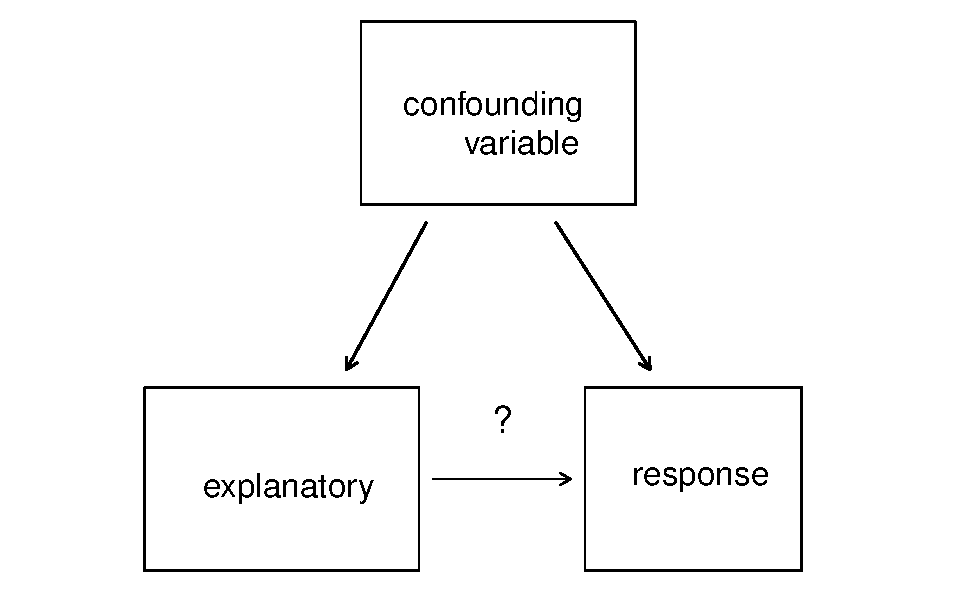
\includegraphics[width=0.4\linewidth]{02-L01-random-assignment_files/figure-latex/unnamed-chunk-1-1} \end{center}

\begin{enumerate}
\def\labelenumi{\arabic{enumi}.}
\setcounter{enumi}{14}
\item
  \textbf{What is the purpose of random assignment of the subjects in a study to the explanatory variable groups?}
  \vspace{0.8in}
\item
  Suppose in this study on atrial fibrillation, the scientists did randomly assign groups and found that the drug group has a higher proportion of subjects whose heart rates stabilized than the placebo group. Can the scientists conclude the new drug \emph{caused} the increased chance of stabilization? Explain your answer.
  \vspace{0.5in}
\end{enumerate}

\newpage

\begin{enumerate}
\def\labelenumi{\arabic{enumi}.}
\setcounter{enumi}{16}
\tightlist
\item
  \textbf{Both the sampling method (which we covered earlier this week) and the study design will help to determine the \emph{scope of inference} for a study: To \emph{whom} can we generalize, and can we conclude \emph{causation or only association}? Use the table below to determine the scope of inference of this trial study described in question 16.}
  \vspace{0.3in}
\end{enumerate}

\begin{center}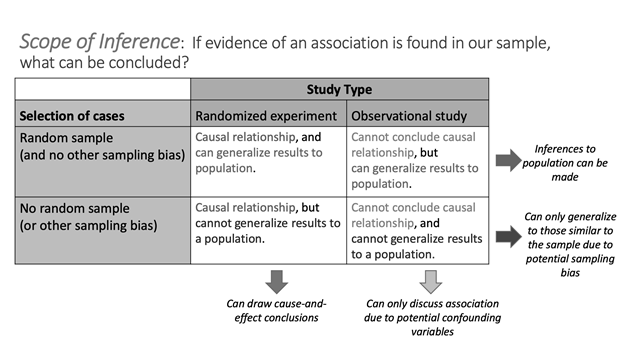
\includegraphics[width=0.75\linewidth]{images/ScopeOfInferenceGreyscale} \end{center}

\begin{enumerate}
\def\labelenumi{\arabic{enumi}.}
\setcounter{enumi}{17}
\item
  Use the table to determine the scope of inference for the study in question 1.
  \vspace{0.3in}
\item
  Use the table to determine the scope of inference for the study in question 2.
  \vspace{0.3in}
\end{enumerate}

\hypertarget{take-home-messages-3}{%
\subsection{Take-home messages}\label{take-home-messages-3}}

\begin{enumerate}
\def\labelenumi{\arabic{enumi}.}
\item
  The study design (observational study vs, experiment) determines if we can draw causal inferences or not. If an association is detected, a randomized experiment allows us to conclude that there is a causal (cause-and-effect) relationship between the explanatory and response variable. Observational studies have potential confounding variables within the study that prevent us from inferring a causal relationship between the variables studied.
\item
  Confounding variables are variables not included in the study that are related to both the explanatory and the response variables. When there are potential confounding variables in the study we cannot draw causal inferences.
\item
  Random assignment balances confounding variables across treatment groups. This eliminates any possible confounding variables by breaking the connections between the explanatory variable and the potential confounding variables.
\item
  Observational studies will always carry the possibility of confounding variables. Randomized experiments, which use random assignment, will have no confounding variables.
\end{enumerate}

\newpage

\hypertarget{additional-notes-3}{%
\subsection{Additional notes}\label{additional-notes-3}}

Use this space to summarize your thoughts and take additional notes on today's activity and material covered.

\newpage

\hypertarget{out-of-class-activity-4-movie-profits-correlation-and-coefficient-of-determination}{%
\section{Out of Class Activity 4: Movie Profits --- Correlation and Coefficient of Determination}\label{out-of-class-activity-4-movie-profits-correlation-and-coefficient-of-determination}}

\setstretch{1}

\hypertarget{learning-outcomes-4}{%
\subsection{Learning outcomes}\label{learning-outcomes-4}}

\begin{itemize}
\item
  Identify and create appropriate summary statistics and plots
  given a data set with two quantitative variables.
\item
  Calculate and interpret \(R^2\), the coefficient of determination, in context of the problem.
\item
  Find the correlation coefficient from \texttt{R} output or from \(R^2\) and the sign of the slope.
\end{itemize}

\hypertarget{terminology-review-4}{%
\subsection{Terminology review}\label{terminology-review-4}}

In today's activity, we will review summary measures and plots for two quantitative variables. Some terms covered in this activity are:

\begin{itemize}
\item
  Correlation (\(r\) or \(R\))
\item
  Coefficient of determination (\(r\)-squared or \(R^2\))
\end{itemize}

To review these concepts, see Chapter 3 in the textbook.

\hypertarget{movies-released-in-2016}{%
\subsection{Movies released in 2016}\label{movies-released-in-2016}}

A data set was collected on movies released in 2016 ({``{IMDb} Movies Extensive Dataset''} 2016). Here is a list of some of the variables collected on the observational units, movies released in 2016.

\begin{longtable}[]{@{}
  >{\raggedright\arraybackslash}p{(\columnwidth - 2\tabcolsep) * \real{0.2353}}
  >{\raggedright\arraybackslash}p{(\columnwidth - 2\tabcolsep) * \real{0.7647}}@{}}
\toprule()
\begin{minipage}[b]{\linewidth}\raggedright
\textbf{Variable}
\end{minipage} & \begin{minipage}[b]{\linewidth}\raggedright
\textbf{Description}
\end{minipage} \\
\midrule()
\endhead
\texttt{budget\_mil} & Amount of money (in US \$ millions) budgeted for the production of the movie \\
\texttt{revenue\_mil} & Amount of money (in US \$ millions) the movie made after release \\
\texttt{duration} & Length of the movie (in minutes) \\
\texttt{content\_rating} & Rating of the movie (\texttt{G}, \texttt{PG}, \texttt{PG-13}, \texttt{R}, \texttt{Not\ Rated}) \\
\texttt{imdb\_score} & IMDb user rating score from 1 to 10 \\
\texttt{genres} & Categories the movie falls into (e.g., Action, Drama, etc.) \\
\texttt{facebook\_likes} & Number of likes a movie receives on Facebook \\
\bottomrule()
\end{longtable}

\newpage

\hypertarget{correlation}{%
\subsubsection*{Correlation}\label{correlation}}
\addcontentsline{toc}{subsubsection}{Correlation}

Correlation measures the strength and the direction of the linear relationship between two quantitative variables. The closer the value of correlation to \(+1\) or \(-1\), the stronger the linear relationship. Values close to zero indicate a very weak linear relationship between the two variables. The following output shows a correlation matrix between several pairs of quantitative variables. Upload and open the Movie Profits Out of Class Activity F22 Code \texttt{R} script file. Highlight and run lines 1--12. Highlight and run lines 1--12 to produce the same table as below.

\begin{Shaded}
\begin{Highlighting}[]
\NormalTok{movies }\OtherTok{\textless{}{-}} \FunctionTok{read.csv}\NormalTok{(}\StringTok{"https://math.montana.edu/courses/s216/data/Movies2016.csv"}\NormalTok{) }\CommentTok{\# Reads in data set}
\NormalTok{movies }\SpecialCharTok{\%\textgreater{}\%}  \CommentTok{\# Data set pipes into}
  \FunctionTok{select}\NormalTok{(}\FunctionTok{c}\NormalTok{(}\StringTok{"budget\_mil"}\NormalTok{, }\StringTok{"revenue\_mil"}\NormalTok{, }
           \StringTok{"duration"}\NormalTok{, }\StringTok{"imdb\_score"}\NormalTok{, }
           \StringTok{"facebook\_likes"}\NormalTok{)) }\SpecialCharTok{\%\textgreater{}\%}
  \FunctionTok{cor}\NormalTok{(}\AttributeTok{use=}\StringTok{"pairwise.complete.obs"}\NormalTok{) }\SpecialCharTok{\%\textgreater{}\%}
  \FunctionTok{round}\NormalTok{(}\DecValTok{3}\NormalTok{)}
\end{Highlighting}
\end{Shaded}

\begin{verbatim}
#>                budget_mil revenue_mil duration imdb_score facebook_likes
#> budget_mil          1.000       0.686    0.463      0.292          0.678
#> revenue_mil         0.686       1.000    0.227      0.398          0.723
#> duration            0.463       0.227    1.000      0.261          0.438
#> imdb_score          0.292       0.398    0.261      1.000          0.309
#> facebook_likes      0.678       0.723    0.438      0.309          1.000
\end{verbatim}

\begin{enumerate}
\def\labelenumi{\arabic{enumi}.}
\tightlist
\item
  Using the output above, which two variables have the \emph{strongest} correlation? What is the value of this correlation?
\end{enumerate}

\vspace{0.5in}

\begin{enumerate}
\def\labelenumi{\arabic{enumi}.}
\setcounter{enumi}{1}
\tightlist
\item
  What is the value of correlation between budget and revenue?
\end{enumerate}

\vspace{0.3in}

\begin{enumerate}
\def\labelenumi{\arabic{enumi}.}
\setcounter{enumi}{2}
\tightlist
\item
  Based on the value of correlation found in question 2, what would the sign of the slope be? Positive or negative? Explain.
\end{enumerate}

\vspace{0.5in}

\begin{enumerate}
\def\labelenumi{\arabic{enumi}.}
\setcounter{enumi}{3}
\tightlist
\item
  Explain why the correlation values on the diagonal are equal to 1.
\end{enumerate}

\vspace{0.8in}
\newpage

\hypertarget{coefficient-of-determination-squared-correlation}{%
\subsubsection*{Coefficient of determination (squared correlation)}\label{coefficient-of-determination-squared-correlation}}
\addcontentsline{toc}{subsubsection}{Coefficient of determination (squared correlation)}

Another summary measure used to explain the linear relationship between two quantitative variables is the coefficient of determination (\(r^2\)). The coefficient of determination, \(r^2\), can also be used to describe the strength of the linear relationship between two quantitative variables. The value of \(r^2\) (a value between 0 and 1) represents the \textbf{proportion of variation in the response that is explained by the least squares line with the explanatory variable}. There are two ways to calculate the coefficient of determination:

~~~Square the correlation coefficient: \(R^2 = (R)^2\)

~~~Use the variances of the response and the residuals: \(R^2 = \dfrac{s_y^2 - s_{RES}^2}{s_y^2} = \dfrac{SST - SSE}{SST}\)

\begin{enumerate}
\def\labelenumi{\arabic{enumi}.}
\setcounter{enumi}{5}
\tightlist
\item
  Use the correlation, \(R\), found in question 2 of the activity, to calculate the coefficient of determination between budget and revenue, \(R^2\).
\end{enumerate}

\vspace{.4in}

\begin{enumerate}
\def\labelenumi{\arabic{enumi}.}
\setcounter{enumi}{6}
\tightlist
\item
  The variance of the response variable, revenue in \$MM, is about \(s_{revenue}^2 = 8024.261\) \$MM\(^2\) and the variability in the residuals is about \(s_{RES}^2 = 4244.832\) \$MM\(^2\). Use these values to calculate the coefficient of determination. Verify that your answers to 6 and 7 are the same.
\end{enumerate}

\vspace{1in}

In the next part of the activity we will explore what the coefficient of determination measures.

In Figure \ref{fig:horizontal-line}, we see the data plotted with a horizontal line. Note that the line has a slope of zero, this shows no relationship between budget and revenue.

\begin{figure}

{\centering 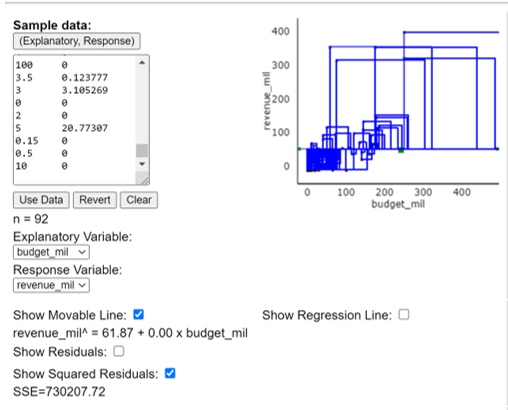
\includegraphics[width=0.5\linewidth]{images/HorizontalLine} 

}

\caption{Plot of the data with no slope.}\label{fig:horizontal-line}
\end{figure}

\begin{enumerate}
\def\labelenumi{\arabic{enumi}.}
\setcounter{enumi}{7}
\tightlist
\item
  Write down the value of SSE given in this image. Since this is the sum of squared errors (SSE) for the horizontal line we call this the total sum of squares (SST).
\end{enumerate}

\vspace{0.2in}

In Figure \ref{fig:regression-line}, we see the data plotted with the regression line (we will learn more about the regression line in the next class). This is the line of best fit between budget and revenue.

\begin{figure}

{\centering 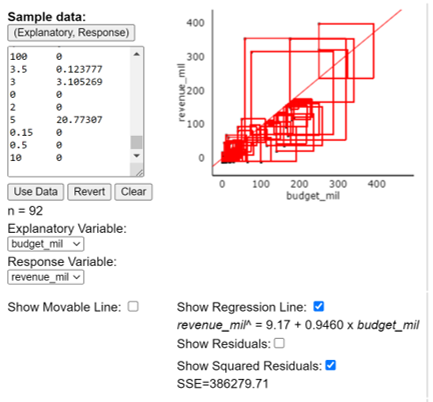
\includegraphics[width=0.5\linewidth]{images/Regression_Line} 

}

\caption{Plot of the data showing the regression line.}\label{fig:regression-line}
\end{figure}

\begin{enumerate}
\def\labelenumi{\arabic{enumi}.}
\setcounter{enumi}{8}
\tightlist
\item
  Write down the value for SSE from this image.
\end{enumerate}

\vspace{0.2in}

\begin{enumerate}
\def\labelenumi{\arabic{enumi}.}
\setcounter{enumi}{9}
\tightlist
\item
  Calculate the value for \(R^2\) using the values found for SST and SSE.
\end{enumerate}

\vspace{1in}

\begin{enumerate}
\def\labelenumi{\arabic{enumi}.}
\setcounter{enumi}{10}
\tightlist
\item
  Write a sentence interpreting the coefficient of determination in context of the problem.
\end{enumerate}

\newpage

\hypertarget{take-home-messages-4}{%
\subsection{Take-home messages}\label{take-home-messages-4}}

\begin{enumerate}
\def\labelenumi{\arabic{enumi}.}
\item
  The sign of correlation and the sign of the slope will always be the same. The closer the value of correlation is to \(-1\) or \(+1\), the stronger the relationship between the explanatory and the response variable.
\item
  The coefficient of determination multiplied by 100 (\(R^2 \times 100\)) measures the percent of variation in the response variable that is explained by the relationship with the explanatory variable. The closer the value of the coefficient of determination is to 100\%, the stronger the relationship.
\end{enumerate}

\hypertarget{additional-notes-4}{%
\subsection{Additional notes}\label{additional-notes-4}}

Use this space to summarize your thoughts and take additional notes on today's activity and material covered.

\newpage

\hypertarget{activity-4-movie-profits-linear-regression}{%
\section{Activity 4: Movie Profits --- Linear Regression}\label{activity-4-movie-profits-linear-regression}}

\setstretch{1}

\hypertarget{learning-outcomes-5}{%
\subsection{Learning outcomes}\label{learning-outcomes-5}}

\begin{itemize}
\item
  Identify and create appropriate summary statistics and plots
  given a data set with two quantitative variables.
\item
  Use scatterplots to assess the relationship between two quantitative variables.
\item
  Find the estimated line of regression using summary statistics and \texttt{R} linear model (\texttt{lm()}) output.
\item
  Interpret the slope coefficient in context of the problem.
\end{itemize}

\hypertarget{terminology-review-5}{%
\subsection{Terminology review}\label{terminology-review-5}}

In today's activity, we will review summary measures and plots for two quantitative variables. Some terms covered in this activity are:

\begin{itemize}
\item
  Scatterplot
\item
  Least-squares line of regression
\item
  Slope and \(y\)-intercept
\item
  Residuals
\end{itemize}

To review these concepts, see Chapter 6 \& 7 in the textbook.

\hypertarget{movies-released-in-2016-1}{%
\subsection{Movies released in 2016}\label{movies-released-in-2016-1}}

We will revisit the movie data set collected on Movies released in 2016 ({``{IMDb} Movies Extensive Dataset''} 2016) to further explore the relationship between budget and revenue. Here is a reminder of the variables collected on these movies.

\begin{longtable}[]{@{}
  >{\raggedright\arraybackslash}p{(\columnwidth - 2\tabcolsep) * \real{0.2353}}
  >{\raggedright\arraybackslash}p{(\columnwidth - 2\tabcolsep) * \real{0.7647}}@{}}
\toprule()
\begin{minipage}[b]{\linewidth}\raggedright
\textbf{Variable}
\end{minipage} & \begin{minipage}[b]{\linewidth}\raggedright
\textbf{Description}
\end{minipage} \\
\midrule()
\endhead
\texttt{budget\_mil} & Amount of money (in US \$ millions) budgeted for the production of the movie \\
\texttt{revenue\_mil} & Amount of money (in US \$ millions) the movie made after release \\
\texttt{duration} & Length of the movie (in minutes) \\
\texttt{content\_rating} & Rating of the movie (\texttt{G}, \texttt{PG}, \texttt{PG-13}, \texttt{R}, \texttt{Not\ Rated}) \\
\texttt{imdb\_score} & IMDb user rating score from 1 to 10 \\
\texttt{genres} & Categories the movie falls into (e.g., Action, Drama, etc.) \\
\texttt{facebook\_likes} & Number of likes a movie receives on Facebook \\
\bottomrule()
\end{longtable}

\begin{Shaded}
\begin{Highlighting}[]
\NormalTok{movies }\OtherTok{\textless{}{-}} \FunctionTok{read.csv}\NormalTok{(}\StringTok{"https://math.montana.edu/courses/s216/data/Movies2016.csv"}\NormalTok{) }\CommentTok{\# Reads in data set }
\end{Highlighting}
\end{Shaded}

\hypertarget{vocabulary-review}{%
\subsubsection*{Vocabulary review}\label{vocabulary-review}}
\addcontentsline{toc}{subsubsection}{Vocabulary review}

To look at the relationship between two quantitative variables we will create a scatterplot with the explanatory variable on the x-axis and the response variable on the y-axis. We can also find three summary measures for the linear relationship between the two variables: regression slope, correlation and the coefficient of determination.

We will look at the relationship between budget and revenue for movies released in 2016. Enter the explanatory variable name, \texttt{budget\_mil}, for \texttt{explanatory} and the response variable name, \texttt{revenue\_mil}, for \texttt{response} at line 7 in the \texttt{R} script file to create the scatterplot. (Note: both variables are measured in ``millions of dollars'' (\$MM).) Upload and open the Movie Profits Activity 4 F22 Code \texttt{R} script file. Highlight and run lines 1--12.

\begin{Shaded}
\begin{Highlighting}[]
\NormalTok{movies }\SpecialCharTok{\%\textgreater{}\%} \CommentTok{\# Data set pipes into...}
\FunctionTok{ggplot}\NormalTok{(}\FunctionTok{aes}\NormalTok{(}\AttributeTok{x =}\NormalTok{ explanatory, }\AttributeTok{y =}\NormalTok{ response))}\SpecialCharTok{+}  \CommentTok{\# Specify variables}
  \FunctionTok{geom\_point}\NormalTok{() }\SpecialCharTok{+}  \CommentTok{\# Add scatterplot of points}
  \FunctionTok{labs}\NormalTok{(}\AttributeTok{x =} \StringTok{"Budget in Millions ($)"}\NormalTok{,  }\CommentTok{\# Label x{-}axis}
       \AttributeTok{y =} \StringTok{"Revenue in Millions ($)"}\NormalTok{,  }\CommentTok{\# Label y{-}axis}
       \AttributeTok{title =} \StringTok{"Revenue vs. Budget"}\NormalTok{) }\SpecialCharTok{+} \CommentTok{\# Be sure to title your plots}
  \FunctionTok{geom\_smooth}\NormalTok{(}\AttributeTok{method =} \StringTok{"lm"}\NormalTok{, }\AttributeTok{se =} \ConstantTok{FALSE}\NormalTok{)  }\CommentTok{\# Add regression line}
\end{Highlighting}
\end{Shaded}

\begin{enumerate}
\def\labelenumi{\arabic{enumi}.}
\tightlist
\item
  Sketch the scatterplot created from the code.
\end{enumerate}

\vspace{2in}

\begin{enumerate}
\def\labelenumi{\arabic{enumi}.}
\setcounter{enumi}{1}
\tightlist
\item
  Assess the four features of the scatterplot that describe this relationship. Describe each feature using a complete sentence!
\end{enumerate}

\begin{itemize}
\tightlist
\item
  Form (linear, non-linear)
\end{itemize}

\vspace{.2in}

\begin{itemize}
\tightlist
\item
  Direction (positive, negative)
\end{itemize}

\vspace{.2in}

\begin{itemize}
\tightlist
\item
  Strength
\end{itemize}

\vspace{.2in}

\begin{itemize}
\tightlist
\item
  Unusual observations or outliers
\end{itemize}

\vspace{.2in}

\begin{enumerate}
\def\labelenumi{\arabic{enumi}.}
\setcounter{enumi}{2}
\tightlist
\item
  Based on the plot, does there appear to be an association between budget and revenue? Explain.
\end{enumerate}

\vspace{1in}

\hypertarget{slope}{%
\subsubsection*{Slope}\label{slope}}
\addcontentsline{toc}{subsubsection}{Slope}

The linear model function in \texttt{R} (\texttt{lm()}) gives us the summary for the least squares regression line. The estimate for \texttt{(Intercept)} is the \(y\)-intercept for the line of least squares, and the estimate for \texttt{budget\_mil} (the \(x\)-variable name) is the value of \(b_1\), the slope. Run lines 16 -- 19 in the \texttt{R} script file to reproduce the linear model output found in the coursepack.

\begin{Shaded}
\begin{Highlighting}[]
\CommentTok{\# Fit linear model: y \textasciitilde{} x}
\NormalTok{revenueLM }\OtherTok{\textless{}{-}} \FunctionTok{lm}\NormalTok{(revenue\_mil }\SpecialCharTok{\textasciitilde{}}\NormalTok{ budget\_mil, }\AttributeTok{data=}\NormalTok{movies)}
\FunctionTok{summary}\NormalTok{(revenueLM)}\SpecialCharTok{$}\NormalTok{coefficients }\CommentTok{\# Display coefficient summary}
\end{Highlighting}
\end{Shaded}

\begin{verbatim}
#>              Estimate Std. Error  t value     Pr(>|t|)
#> (Intercept) 9.1693054  9.0175499 1.016829 3.119606e-01
#> budget_mil  0.9460001  0.1056786 8.951670 4.339561e-14
\end{verbatim}

\begin{enumerate}
\def\labelenumi{\arabic{enumi}.}
\setcounter{enumi}{3}
\tightlist
\item
  Write out the least squares regression line using the summary statistics provided above in context of the problem.
  \vspace{0.8in}
\end{enumerate}

You may remember from middle and high school that slope \(=\frac{\mbox{rise}}{\mbox{run}}\).

Using \(b_1\) to represent slope, we can write that as the fraction \(\frac{b_1}{1}\).

Therefore, the slope predicts how much the line will \emph{rise} for each \emph{run} of +1. In other words, as the \(x\) variable increases by 1 unit, the \(y\) variable is predicted to change (increase/decrease) by the value of slope.

\begin{enumerate}
\def\labelenumi{\arabic{enumi}.}
\setcounter{enumi}{4}
\tightlist
\item
  Interpret the value of slope in context of the problem.
\end{enumerate}

\vspace{.8in}

\begin{enumerate}
\def\labelenumi{\arabic{enumi}.}
\setcounter{enumi}{5}
\tightlist
\item
  Using the least squares line from question 4, predict the revenue for a movie with a budget of 165 \$MM.
\end{enumerate}

\vspace{.6in}

\begin{enumerate}
\def\labelenumi{\arabic{enumi}.}
\setcounter{enumi}{6}
\tightlist
\item
  Predict the revenue for a movie with a budget of 500 \$MM.
\end{enumerate}

\vspace{0.8in}

\begin{enumerate}
\def\labelenumi{\arabic{enumi}.}
\setcounter{enumi}{7}
\tightlist
\item
  The prediction in question 7 is an example of what?
\end{enumerate}

\vspace{0.3in}

\hypertarget{residuals}{%
\subsubsection*{Residuals}\label{residuals}}
\addcontentsline{toc}{subsubsection}{Residuals}

The model we are using assumes the relationship between the two variables follows a straight line. The residuals are the errors, or the variability in the response that hasn't been modeled by the line (model).

\begin{center}
Data = Model + Residual

$\implies$ Residual = Data $-$ Model

$e_i=y_i-\hat{y}_i$
\end{center}

\begin{enumerate}
\def\labelenumi{\arabic{enumi}.}
\setcounter{enumi}{8}
\tightlist
\item
  The movie \emph{Independence Day: Resurgence} had a budget of 165 \$MM and revenue of 102.315 \$MM. Find the residual for this movie.
\end{enumerate}

\vspace{.8in}

\begin{enumerate}
\def\labelenumi{\arabic{enumi}.}
\setcounter{enumi}{9}
\tightlist
\item
  Did the line of regression overestimate or underestimate the revenue for this movie?
\end{enumerate}

\vspace{.2in}

\hypertarget{multivariable-plots}{%
\subsubsection*{Multivariable plots}\label{multivariable-plots}}
\addcontentsline{toc}{subsubsection}{Multivariable plots}

What if we wanted to see if the relationship between movie budget and revenue differs if we add another variable into the picture? The following plot visualizes three variables, creating a \textbf{multivariable} plot.

\begin{Shaded}
\begin{Highlighting}[]
\NormalTok{movies }\SpecialCharTok{\%\textgreater{}\%} \CommentTok{\# Data set pipes into...}
  \FunctionTok{filter}\NormalTok{(content\_rating }\SpecialCharTok{!=} \StringTok{"Not Rated"}\NormalTok{) }\SpecialCharTok{\%\textgreater{}\%} \CommentTok{\# Remove Not Rated movies}
  \FunctionTok{ggplot}\NormalTok{(}\FunctionTok{aes}\NormalTok{(}\AttributeTok{x =}\NormalTok{ budget\_mil, }\AttributeTok{y =}\NormalTok{ revenue\_mil, }\AttributeTok{color =}\NormalTok{ content\_rating)) }\SpecialCharTok{+}  \CommentTok{\# Specify variables}
  \FunctionTok{geom\_point}\NormalTok{(}\FunctionTok{aes}\NormalTok{(}\AttributeTok{shape =}\NormalTok{ content\_rating), }\AttributeTok{size =} \DecValTok{3}\NormalTok{) }\SpecialCharTok{+}  \CommentTok{\# Add scatterplot of points}
  \FunctionTok{labs}\NormalTok{(}\AttributeTok{x =} \StringTok{"Budget in Millions ($)"}\NormalTok{,  }\CommentTok{\# Label x{-}axis}
       \AttributeTok{y =} \StringTok{"Revenue in Millions ($)"}\NormalTok{,  }\CommentTok{\# Label y{-}axis}
       \AttributeTok{color =} \StringTok{"content\_rating"}\NormalTok{,  }\CommentTok{\# Label legend}
       \AttributeTok{title =} \StringTok{"Revenue vs. Budget"}\NormalTok{) }\SpecialCharTok{+} \CommentTok{\# Be sure to tile your plots}
  \FunctionTok{geom\_smooth}\NormalTok{(}\AttributeTok{method =} \StringTok{"lm"}\NormalTok{, }\AttributeTok{se =} \ConstantTok{FALSE}\NormalTok{, }\AttributeTok{lwd =} \DecValTok{2}\NormalTok{) }\SpecialCharTok{+} \CommentTok{\# Add regression lines}
  \FunctionTok{scale\_color\_grey}\NormalTok{() }\CommentTok{\# Make black and white}
\end{Highlighting}
\end{Shaded}

\begin{center}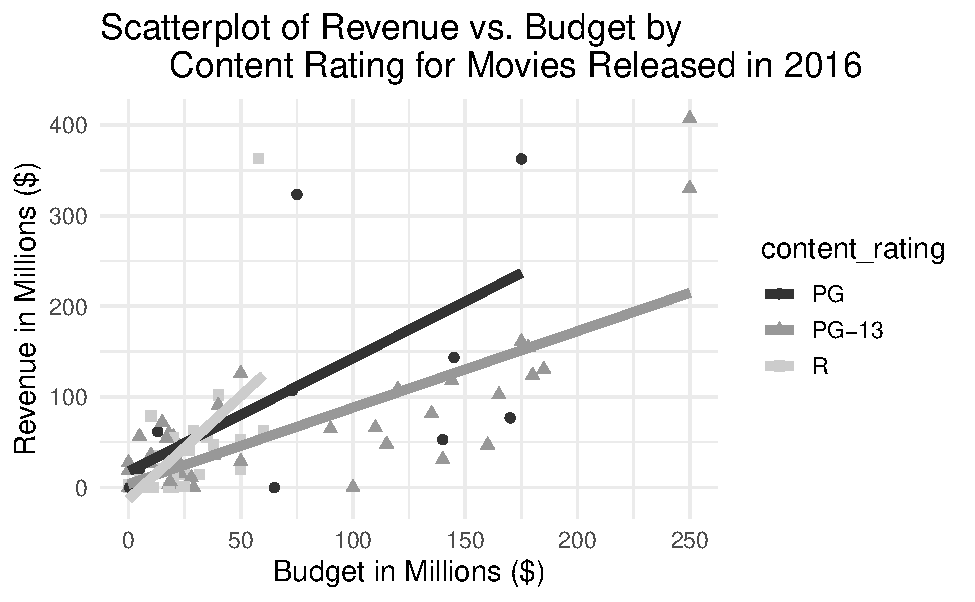
\includegraphics[width=0.7\linewidth]{04-A04-EDA-two-quantitative-LR_files/figure-latex/unnamed-chunk-4-1} \end{center}

\begin{enumerate}
\def\labelenumi{\arabic{enumi}.}
\setcounter{enumi}{10}
\tightlist
\item
  Identify the three variables plotted in this graph.
\end{enumerate}

\vspace{0.5in}

\begin{enumerate}
\def\labelenumi{\arabic{enumi}.}
\setcounter{enumi}{11}
\tightlist
\item
  Does the \emph{relationship} between movie budget and revenue differ among the different content ratings? Explain.
\end{enumerate}

\vspace{0.8in}
\newpage

\hypertarget{take-home-messages-5}{%
\subsection{Take-home messages}\label{take-home-messages-5}}

\begin{enumerate}
\def\labelenumi{\arabic{enumi}.}
\item
  Two quantitative variables are graphically displayed in a scatterplot. The explanatory variable is on the \(x\)-axis and the response variable is on the \(y\)-axis. When describing the relationship between two quantitative variables we look at the form (linear or non-linear), direction (positive or negative), strength, and for the presence of outliers.
\item
  There are three summary statistics used to summarize the relationship between two quantitative variables: correlation (\(R\)), slope of the regression line (\(b_1\)), and the coefficient of determination (\(R^2\)).
\item
  We can use the line of regression to predict values of the response variable for values of the explanatory variable. Do not use values of the explanatory variable that are outside of the range of values in the data set to predict values of the response variable (reflect on why this is true.). This is called \textbf{extrapolation}.
\end{enumerate}

\hypertarget{additional-notes-5}{%
\subsection{Additional notes}\label{additional-notes-5}}

Use this space to summarize your thoughts and take additional notes on today's activity and material covered.

\newpage

\hypertarget{week-4-lab-penguins}{%
\section{Week 4 Lab: Penguins}\label{week-4-lab-penguins}}

\setstretch{1}

\hypertarget{learning-outcomes-6}{%
\subsection{Learning outcomes}\label{learning-outcomes-6}}

\begin{itemize}
\item
  Identify and create appropriate summary statistics and plots
  given a data set with two quantitative variables.
\item
  Use scatterplots to assess the relationship between two quantitative variables.
\item
  Find the estimated line of regression using summary statistics and R linear model (\texttt{lm()}) output.
\item
  Interpret the slope coefficient in context of the problem.
\item
  Calculate and interpret \(R^2\), the coefficient of determination, in context of the problem.
\item
  Find the correlation coefficient from R output or from \(R^2\) and the sign of the slope.
\end{itemize}

\hypertarget{penguins}{%
\subsection{Penguins}\label{penguins}}

The Palmer Station Long Term Ecological Research Program sampled three penguin species on islands in the Palmer Archipelago in Antarctica. Researchers took various body measurements on the penguins, including flipper length and body mass. The researchers were interested in the relationship between flipper length and body mass and wondered if flipper length could be used to accurately predict the body mass of these three penguin species.

Upload and import the \texttt{Antarctica\_Penguins} csv file and the provided R script file for week 4 lab. Enter the name of the data set (see the environment tab) for \texttt{datasetname} in the R script file in line 4.

First we will create a scatterplot of the flipper length and body mass. Notice that we are using flipper length to predict body mass. This makes flipper length the explanatory variable. \textbf{Make sure to give your plot a descriptive title.} Highlight and run lines 1--13 in the R script file. \textbf{Upload a copy of your scatterplot to Gradescope.}

\begin{Shaded}
\begin{Highlighting}[]
\NormalTok{penguins }\OtherTok{\textless{}{-}}\NormalTok{ datasetname }\CommentTok{\#Creates the object penguins}
\NormalTok{penguins }\SpecialCharTok{\%\textgreater{}\%}
  \FunctionTok{ggplot}\NormalTok{(}\FunctionTok{aes}\NormalTok{(}\AttributeTok{x =}\NormalTok{ flipper\_length\_mm, }\AttributeTok{y =}\NormalTok{ body\_mass\_g))}\SpecialCharTok{+}  \CommentTok{\# Specify variables}
  \FunctionTok{geom\_point}\NormalTok{() }\SpecialCharTok{+}  \CommentTok{\# Add scatterplot of points}
  \FunctionTok{labs}\NormalTok{(}\AttributeTok{x =} \StringTok{"flipper length (mm)"}\NormalTok{,  }\CommentTok{\# Label x{-}axis}
       \AttributeTok{y =} \StringTok{"body mass (g)"}\NormalTok{,  }\CommentTok{\# Label y{-}axis}
       \AttributeTok{title =} \StringTok{"Title"}\NormalTok{) }\SpecialCharTok{+} \CommentTok{\# Be sure to title your plots}
  \FunctionTok{geom\_smooth}\NormalTok{(}\AttributeTok{method =} \StringTok{"lm"}\NormalTok{, }\AttributeTok{se =} \ConstantTok{FALSE}\NormalTok{)  }\CommentTok{\# Add regression line}
\end{Highlighting}
\end{Shaded}

\begin{enumerate}
\def\labelenumi{\arabic{enumi}.}
\tightlist
\item
  Assess the four features of the scatterplot that describe this relationship.
  \vspace{1mm}
\end{enumerate}

\begin{itemize}
\tightlist
\item
  Form (linear, non-linear)
\end{itemize}

\vspace{.1in}

\begin{itemize}
\tightlist
\item
  Direction (positive, negative)
\end{itemize}

\vspace{.1in}

\begin{itemize}
\tightlist
\item
  Strength
\end{itemize}

\vspace{.1in}

\begin{itemize}
\tightlist
\item
  Unusual observations or outliers
\end{itemize}

\vspace{.1in}

Highlight and run lines 16--20 to get the correlation matrix in the R script file.

\begin{Shaded}
\begin{Highlighting}[]
\NormalTok{penguins }\SpecialCharTok{\%\textgreater{}\%}  \CommentTok{\# Data set pipes into}
  \FunctionTok{select}\NormalTok{(}\FunctionTok{c}\NormalTok{(}\StringTok{"bill\_length\_mm"}\NormalTok{, }\StringTok{"bill\_depth\_mm"}\NormalTok{, }
           \StringTok{"flipper\_length\_mm"}\NormalTok{, }\StringTok{"body\_mass\_g"}\NormalTok{)) }\SpecialCharTok{\%\textgreater{}\%}
  \FunctionTok{cor}\NormalTok{(}\AttributeTok{use=}\StringTok{"pairwise.complete.obs"}\NormalTok{) }\SpecialCharTok{\%\textgreater{}\%}
  \FunctionTok{round}\NormalTok{(}\DecValTok{3}\NormalTok{)}
\end{Highlighting}
\end{Shaded}

\begin{enumerate}
\def\labelenumi{\arabic{enumi}.}
\setcounter{enumi}{1}
\tightlist
\item
  Using the R output, which two variables have the \emph{strongest} correlation? What is the value of this correlation?
\end{enumerate}

\vspace{0.5in}

\begin{enumerate}
\def\labelenumi{\arabic{enumi}.}
\setcounter{enumi}{2}
\tightlist
\item
  Using the value of correlation found in question 2, calculate the value of the coefficient of determination.
\end{enumerate}

\vspace{0.5in}

\begin{enumerate}
\def\labelenumi{\arabic{enumi}.}
\setcounter{enumi}{3}
\tightlist
\item
  \textbf{Interpret the coefficient of determination in context of the problem.}
\end{enumerate}

\vspace{1in}

Enter the variable \texttt{body\_mass\_g} for \texttt{response} and the variable name \texttt{flipper\_length\_mm} for \texttt{explanatory} in line 23 in the R script file. Highlight and run lines 23--24 to get the linear model output.

\begin{Shaded}
\begin{Highlighting}[]
\CommentTok{\# Fit linear model: y \textasciitilde{} x}
\NormalTok{penguinsLM }\OtherTok{\textless{}{-}} \FunctionTok{lm}\NormalTok{(response}\SpecialCharTok{\textasciitilde{}}\NormalTok{explanatory, }\AttributeTok{data=}\NormalTok{penguins)}
\FunctionTok{summary}\NormalTok{(penguinsLM)}\SpecialCharTok{$}\NormalTok{coefficients }\CommentTok{\# Display coefficient summary}
\end{Highlighting}
\end{Shaded}

\begin{enumerate}
\def\labelenumi{\arabic{enumi}.}
\setcounter{enumi}{4}
\tightlist
\item
  Write out the least squares regression line using the summary statistics from the R output in context of the problem.
\end{enumerate}

\vspace{.5in}

\begin{enumerate}
\def\labelenumi{\arabic{enumi}.}
\setcounter{enumi}{5}
\tightlist
\item
  \textbf{Interpret the value of slope in context of the problem.}
\end{enumerate}

\vspace{.8in}

\begin{enumerate}
\def\labelenumi{\arabic{enumi}.}
\setcounter{enumi}{6}
\tightlist
\item
  \textbf{Using the least squares regression line from question 5, predict the body mass for a penguin with a flipper length of 181 mm.}
\end{enumerate}

\vspace{.6in}

\begin{enumerate}
\def\labelenumi{\arabic{enumi}.}
\setcounter{enumi}{7}
\tightlist
\item
  One penguin had a flipper length of 181 mm and a body mass of 3750 g. Find the residual for this penguin.
\end{enumerate}

\vspace{.8in}

\begin{enumerate}
\def\labelenumi{\arabic{enumi}.}
\setcounter{enumi}{8}
\tightlist
\item
  Did the line of regression overestimate or underestimate the body mass for this penguin?
\end{enumerate}

\vspace{0.5in}

Highlight and run lines 27--34 to get the multivariate plot.

\begin{Shaded}
\begin{Highlighting}[]
\NormalTok{penguins }\SpecialCharTok{\%\textgreater{}\%}
  \FunctionTok{ggplot}\NormalTok{(}\FunctionTok{aes}\NormalTok{(}\AttributeTok{x =}\NormalTok{ flipper\_length\_mm, }\AttributeTok{y =}\NormalTok{ body\_mass\_g, }\AttributeTok{color=}\NormalTok{species))}\SpecialCharTok{+}  \CommentTok{\# Specify variables}
  \FunctionTok{geom\_point}\NormalTok{(}\FunctionTok{aes}\NormalTok{(}\AttributeTok{shape =}\NormalTok{ species), }\AttributeTok{size =} \DecValTok{3}\NormalTok{) }\SpecialCharTok{+}  \CommentTok{\# Add scatterplot of points}
  \FunctionTok{labs}\NormalTok{(}\AttributeTok{x =} \StringTok{"flipper length (mm)"}\NormalTok{,  }\CommentTok{\# Label x{-}axis}
       \AttributeTok{y =} \StringTok{"body mass (g)"}\NormalTok{,  }\CommentTok{\# Label y{-}axis}
       \AttributeTok{color =} \StringTok{"species"}\NormalTok{,}
       \AttributeTok{title =} \StringTok{"TITLE"}\NormalTok{) }\SpecialCharTok{+} \CommentTok{\# Be sure to tile your plots}
  \FunctionTok{geom\_smooth}\NormalTok{(}\AttributeTok{method =} \StringTok{"lm"}\NormalTok{, }\AttributeTok{se =} \ConstantTok{FALSE}\NormalTok{)  }\CommentTok{\# Add regression line}
\end{Highlighting}
\end{Shaded}

\begin{enumerate}
\def\labelenumi{\arabic{enumi}.}
\setcounter{enumi}{9}
\tightlist
\item
  What three variables are plotted on this plot?
\end{enumerate}

\vspace{0.3in}

\begin{enumerate}
\def\labelenumi{\arabic{enumi}.}
\setcounter{enumi}{10}
\tightlist
\item
  \textbf{Does adding the variable species affect the relationship between body mass and flipper length? Explain your answer.}
\end{enumerate}

\newpage

\hypertarget{exam-1-review}{%
\chapter{Exam 1 Review}\label{exam-1-review}}

Use the provided data set from the Islands (ExamReviewData.csv) and the appropriate Exam 1 Review R script file to answer the following questions. Each adult (\textgreater21) islander was selected at random from all adult islanders. Variables and their descriptions are listed below. Music type (classical or heavy metal) was randomly assigned to the Islanders. Time to complete the puzzle cube was measured after listening to music for each Islander. Heart rate and blood glucose levels were both measured before and then after drinking a caffeinated beverage.

\begin{longtable}[]{@{}
  >{\raggedright\arraybackslash}p{(\columnwidth - 2\tabcolsep) * \real{0.2353}}
  >{\raggedright\arraybackslash}p{(\columnwidth - 2\tabcolsep) * \real{0.7647}}@{}}
\toprule()
\begin{minipage}[b]{\linewidth}\raggedright
\textbf{Variable}
\end{minipage} & \begin{minipage}[b]{\linewidth}\raggedright
\textbf{Description}
\end{minipage} \\
\midrule()
\endhead
\texttt{Island} & Name of Island that the Islander resides on \\
\texttt{City} & Name of City in which the Islander resides \\
\texttt{Population} & Population of the City \\
\texttt{Name} & Name of Islander \\
\texttt{Consent} & Whether the Islander consented to be in the study \\
\texttt{Gender} & Gender of Islander (M = male, F = Female) \\
\texttt{Age} & Age of Islander \\
\texttt{Married} & Marital status of Islander \\
\texttt{Smoking\_Status} & Whether the Islander is a current smoker \\
\texttt{Children} & Whether the Islander has children \\
\texttt{weight\_kg} & Weight measured in kg \\
\texttt{height\_cm} & Height measured in cm \\
\texttt{respiratory\_rate} & Breaths per minute \\
\texttt{Type\_of\_Music} & Music type (Classical or Heavy Medal) Islander was randomly assigned to listen to \\
\texttt{After\_PuzzleCube} & Time to complete puzzle cube (minutes) after listening to assigned music \\
\texttt{Education\_Level} & Highest level of education completed \\
\texttt{Balance\_Test} & Time balanced measured in seconds with eyes closed \\
\texttt{Blood\_Glucose\_before} & Level of blood glucose (mg/dL) before consuming assigned drink \\
\texttt{Heart\_Rate\_before} & Heart rate (bpm) before consuming assigned drink \\
\texttt{Blood\_Glucose\_after} & Level of blood glucose (mg/dL) after consuming assigned drink \\
\texttt{Heart\_Rate\_after} & Heart rate (bpm) after consuming assigned drink \\
\texttt{Diff\_Heart\_Rate} & Difference in heart rate (bpm) for Before - After consuming assigned drink \\
\texttt{Diff\_Blood\_Glucose} & Difference in blood glucose (mg/dL) for Before - After consuming assigned drink \\
\bottomrule()
\end{longtable}

\begin{enumerate}
\def\labelenumi{\arabic{enumi}.}
\tightlist
\item
  What are the observational units?
\end{enumerate}

\vspace{0.1in}

\begin{enumerate}
\def\labelenumi{\arabic{enumi}.}
\setcounter{enumi}{1}
\tightlist
\item
  In the table above, indicate which variables are categorical (C) and which variables are quantitative (Q).
\end{enumerate}

\vspace{0.1in}

\begin{enumerate}
\def\labelenumi{\arabic{enumi}.}
\setcounter{enumi}{2}
\tightlist
\item
  What type of bias may be present in this study? Explain.
\end{enumerate}

\vspace{0.5in}

\begin{enumerate}
\def\labelenumi{\arabic{enumi}.}
\setcounter{enumi}{3}
\tightlist
\item
  Use the appropriate Exam 1 Review R script file to find the appropriate summary statistic and graphical display of the data to assess the following research question, ``Is the proportion of married Islanders greater than 50\%?''
\end{enumerate}

\begin{enumerate}
\def\labelenumi{\alph{enumi}.}
\tightlist
\item
  What is the name of the variable to be assessed in this research question?
\end{enumerate}

\vspace{0.1in}

\begin{enumerate}
\def\labelenumi{\alph{enumi}.}
\setcounter{enumi}{1}
\tightlist
\item
  What type of variable (categorical or quantitative) is the variable you identified?
\end{enumerate}

\vspace{0.1in}

\begin{enumerate}
\def\labelenumi{\alph{enumi}.}
\setcounter{enumi}{2}
\tightlist
\item
  Use the R script file to get the counts for each level of the variable. Fill in the following table with the success, failure, variable name, and counts using the values from the R output.
\end{enumerate}

\begingroup
\begin{center}
\setlength{\tabcolsep}{14pt} 
\renewcommand{\arraystretch}{2} 
\begin{tabular}{|p{2in}|p{2in}|}
\hline
 {\textbf{Variable}} & {\textbf{Counts}} \\ 
 & \\ \hline
 Success & \\ 
 &  \\ \hline
 Failure & \\ 
 &  \\ \hline
 Total &  \\ 
 & \\ \hline  
\end{tabular}
\end{center}
\endgroup

\begin{enumerate}
\def\labelenumi{\alph{enumi}.}
\setcounter{enumi}{3}
\tightlist
\item
  Calculate the value of summary statistic to answer the research question. Give appropriate notation.
\end{enumerate}

\vspace{0.3in}

\begin{enumerate}
\def\labelenumi{\alph{enumi}.}
\setcounter{enumi}{4}
\tightlist
\item
  Interpret the value of the summary statistic in context of the problem:
\end{enumerate}

\vspace{0.3in}

\begin{enumerate}
\def\labelenumi{\alph{enumi}.}
\setcounter{enumi}{5}
\tightlist
\item
  What type of graph(s) would be appropriate for this research question?
\end{enumerate}

\vspace{0.1in}

\begin{enumerate}
\def\labelenumi{\alph{enumi}.}
\setcounter{enumi}{6}
\tightlist
\item
  Using the provided R file create a graph of the data. Sketch the graph below:
\end{enumerate}

\vspace{1.8in}

\begin{enumerate}
\def\labelenumi{\alph{enumi}.}
\setcounter{enumi}{7}
\tightlist
\item
  To what group could the results of this study be applied to?
\end{enumerate}

\vspace{0.2in}

\begin{enumerate}
\def\labelenumi{\arabic{enumi}.}
\setcounter{enumi}{4}
\tightlist
\item
  Use the appropriate Exam 1 Review R script file to find the appropriate summary statistic and graphical display of the data to assess the following research question, ``Is there a difference in proportion of Islanders who have children for those who completed high school and those that completed university?'' Use high school - university as the order of subtraction.
\end{enumerate}

\begin{enumerate}
\def\labelenumi{\alph{enumi}.}
\item
  What is the name of the explanatory variable to be assessed in this research question?
  \vspace{0.3in}

  What type of variable (categorical or quantitative) is the variable you identified?
  \vspace{0.3in}
\item
  What is the name of the response variable to be assessed in this research question?
  \vspace{0.3in}

  What type of variable (categorical or quantitative) is the variable you identified?
  \vspace{0.3in}
\item
  Use the R script file to get the counts for each level and combination of variables. Fill in the following table with the variable names, levels of each variable, and counts using the values from the R output.
\end{enumerate}

\begingroup
\setlength{\tabcolsep}{14pt}
\renewcommand{\arraystretch}{2}
\begin{center}
\begin{tabular}{|c|p{1in}|p{1in}|p{1in}|}
\hline
 & \multicolumn{2}{|c|}{\textbf{Explanatory Variable}} & \\ 
 & \multicolumn{2}{|c|}{ } & \\ \hline
\textbf{Response variable} & Group 1 & Group 2 & Total \\
 & & & \\ \hline
 Success & & & \\
 & & & \\ \hline
 Failure & & & \\
 & & & \\ \hline
 Total & & & \\
 & & & \\ \hline
\end{tabular}
\end{center}
\endgroup

\begin{enumerate}
\def\labelenumi{\alph{enumi}.}
\setcounter{enumi}{3}
\tightlist
\item
  Calculate the value of summary statistic to answer the research question. Give appropriate notation.
\end{enumerate}

\newpage

\begin{enumerate}
\def\labelenumi{\alph{enumi}.}
\setcounter{enumi}{4}
\item
  Interpret the value of the summary statistic in context of the problem:
  \vspace{0.5in}
\item
  What type of graph(s) would be appropriate for this research question?
\end{enumerate}

\vspace{0.2in}

\begin{enumerate}
\def\labelenumi{\alph{enumi}.}
\setcounter{enumi}{6}
\tightlist
\item
  Using the provided R file create a graph of the data. Sketch the graph below:
\end{enumerate}

\vspace{2in}

\begin{enumerate}
\def\labelenumi{\alph{enumi}.}
\setcounter{enumi}{7}
\tightlist
\item
  Based on the graph, does there appear to be an association between the two variables? Explain your answer.
\end{enumerate}

\vspace{0.5in}

\begin{enumerate}
\def\labelenumi{\roman{enumi}.}
\tightlist
\item
  Is this an observational study or a randomized experiment? Explain your answer.
\end{enumerate}

\vspace{0.5in}

\begin{enumerate}
\def\labelenumi{\alph{enumi}.}
\setcounter{enumi}{9}
\tightlist
\item
  What is the scope of inference for this study?
\end{enumerate}

\newpage

\begin{enumerate}
\def\labelenumi{\arabic{enumi}.}
\setcounter{enumi}{5}
\tightlist
\item
  Use the appropriate Exam 1 Review R script file to find the appropriate summary statistic and graphical display of the data to assess the following research question: ``Do Islanders who listen to classical music take less time to complete the puzzle cube after listening to the music than for Islanders that listen to heavy metal music?'' Use classical - heavy metal as the order of subtraction.
\end{enumerate}

\begin{enumerate}
\def\labelenumi{\alph{enumi}.}
\item
  What is the name of the explanatory variable to be assessed in this research question?
  \vspace{0.3in}

  What type of variable (categorical or quantitative) is the variable you identified?
  \vspace{0.3in}
\item
  What is the name of the response variable to be assessed in this research question?
  \vspace{0.3in}

  What type of variable (categorical or quantitative) is the variable you identified?
  \vspace{0.3in}
\item
  Use the R script file to get the summary statistics for each level of the explanatory variable. Fill in the following table with the variable name, levels of the variable, and the summary statistics from the R output.
\end{enumerate}

\begingroup
\setlength{\tabcolsep}{14pt}
\renewcommand{\arraystretch}{2}
\begin{center}
\begin{tabular}{|c|p{1in}|p{1in}|}
\hline
 & \multicolumn{2}{|c|}{\textbf{Explanatory Variable}} \\
 & \multicolumn{2}{|c|}{ } \\ \hline
\textbf{Summary value} & Group 1 & Group 2 \\
 & & \\ \hline
 Mean & & \\ \hline
 Standard deviation & & \\ \hline
 Sample size & & \\ \hline
\end{tabular}
\end{center}
\endgroup

\begin{enumerate}
\def\labelenumi{\alph{enumi}.}
\setcounter{enumi}{3}
\tightlist
\item
  Calculate the value of the summary statistic to answer the research question. Give appropriate notation.
\end{enumerate}

\newpage

\begin{enumerate}
\def\labelenumi{\alph{enumi}.}
\setcounter{enumi}{4}
\tightlist
\item
  Interpret the value of the summary statistic in context of the problem:
\end{enumerate}

\vspace{0.4in}

\begin{enumerate}
\def\labelenumi{\alph{enumi}.}
\setcounter{enumi}{5}
\tightlist
\item
  What type of graph(s) would be appropriate for this research question?
\end{enumerate}

\vspace{0.2in}

\begin{enumerate}
\def\labelenumi{\alph{enumi}.}
\setcounter{enumi}{6}
\tightlist
\item
  Using the provided R file create a graph of the data. Sketch the graph below:
\end{enumerate}

\vspace{2in}

\begin{enumerate}
\def\labelenumi{\alph{enumi}.}
\setcounter{enumi}{7}
\tightlist
\item
  Based on the graph, does there appear to be an association between the two variables? Explain your answer.
\end{enumerate}

\vspace{0.8in}

\begin{enumerate}
\def\labelenumi{\roman{enumi}.}
\item
  Compare the two plots using the four characteristics to describe plots of quantitative variables.
  \vspace{0.1in}

  Shape:
  \vspace{0.2in}

  Center:
  \vspace{0.2in}

  Spread:
  \vspace{0.2in}

  Outliers:
  \vspace{0.2in}
\end{enumerate}

\begin{enumerate}
\def\labelenumi{\alph{enumi}.}
\setcounter{enumi}{9}
\tightlist
\item
  Is this an observational study or a randomized experiment? Explain your answer.
\end{enumerate}

\vspace{0.5in}

\begin{enumerate}
\def\labelenumi{\alph{enumi}.}
\setcounter{enumi}{10}
\tightlist
\item
  What is the scope of inference for this study?
\end{enumerate}

\newpage

\begin{enumerate}
\def\labelenumi{\arabic{enumi}.}
\setcounter{enumi}{6}
\tightlist
\item
  Use the appropriate Exam 1 Review R script file to find the appropriate summary statistic and graphical display of the data to assess the following research question: ``Do Islanders who are heavier tend to take more breaths per minute?''
\end{enumerate}

\begin{enumerate}
\def\labelenumi{\alph{enumi}.}
\item
  What is the name of the explanatory variable to be assessed in this research question?
  \vspace{0.3in}

  What type of variable (categorical or quantitative) is the variable you identified?
  \vspace{0.3in}
\item
  What is the name of the response variable to be assessed in this research question?
  \vspace{0.3in}

  What type of variable (categorical or quantitative) is the variable you identified?
  \vspace{0.3in}
\item
  Use the R script file to get the summary statistics for this data. Fill in the following table using the values from the R output:
\end{enumerate}

\begingroup
\setlength{\tabcolsep}{14pt}
\renewcommand{\arraystretch}{2}
\begin{center}
\begin{tabular}{|c|p{1in}|p{1in}|p{1in}|}
\hline
 & y-intercept & slope & correlation \\ \hline
 \textbf{Summary value} & & & \\ \hline
\end{tabular}
\end{center}
\endgroup

\begin{enumerate}
\def\labelenumi{\alph{enumi}.}
\setcounter{enumi}{3}
\tightlist
\item
  Interpret the value of slope in context of the problem.
\end{enumerate}

\vspace{0.3in}

\begin{enumerate}
\def\labelenumi{\alph{enumi}.}
\setcounter{enumi}{4}
\tightlist
\item
  Interpret the value of correlation in context of the problem.
\end{enumerate}

\vspace{0.2in}

\begin{enumerate}
\def\labelenumi{\alph{enumi}.}
\setcounter{enumi}{5}
\tightlist
\item
  Calculate the value of the coefficient of determination.
\end{enumerate}

\vspace{0.2in}

\begin{enumerate}
\def\labelenumi{\alph{enumi}.}
\setcounter{enumi}{6}
\tightlist
\item
  Interpret the coefficient of determination in context of the problem.
\end{enumerate}

\vspace{0.3in}

\begin{enumerate}
\def\labelenumi{\alph{enumi}.}
\setcounter{enumi}{7}
\tightlist
\item
  What type of graph(s) would be appropriate for this research question?
\end{enumerate}

\newpage

\begin{enumerate}
\def\labelenumi{\roman{enumi}.}
\tightlist
\item
  Using the provided R file create a graph of the data. Sketch the graph below:
\end{enumerate}

\vspace{2in}

\begin{enumerate}
\def\labelenumi{\alph{enumi}.}
\setcounter{enumi}{9}
\tightlist
\item
  Based on the graph, does there appear to be an association between the two variables? Explain your answer.
\end{enumerate}

\vspace{0.8in}

\begin{enumerate}
\def\labelenumi{\alph{enumi}.}
\setcounter{enumi}{10}
\item
  Describe the plot using the four characteristics to describe scatterplots.
  \vspace{0.1in}

  Form:
  \vspace{0.2in}

  Direction:
  \vspace{0.2in}

  Strength:
  \vspace{0.2in}

  Outliers:
  \vspace{0.2in}
\item
  Is this an observational study or a randomized experiment? Explain your answer.
\end{enumerate}

\vspace{0.5in}

\begin{enumerate}
\def\labelenumi{\alph{enumi}.}
\setcounter{enumi}{12}
\tightlist
\item
  What is the scope of inference for this study?
\end{enumerate}

\newpage

\hypertarget{out-of-class-activity-6-helperer-hinderer-simulation-based-hypothesis-test}{%
\section{Out of Class Activity 6: Helperer-Hinderer --- Simulation-based Hypothesis Test}\label{out-of-class-activity-6-helperer-hinderer-simulation-based-hypothesis-test}}

\setstretch{1}

\hypertarget{learning-outcomes-7}{%
\subsection{Learning outcomes}\label{learning-outcomes-7}}

\begin{itemize}
\item
  Identify the two possible explanations (one assuming the null hypothesis and one assuming the alternative hypothesis) for a relationship seen in sample data.
\item
  Given a research question involving a single categorical variable, construct the null and alternative hypotheses
  in words and using appropriate statistical symbols.
\item
  Describe and perform a simulation-based hypothesis test for a single proportion.
\end{itemize}

\hypertarget{terminology-review-6}{%
\subsection{Terminology review}\label{terminology-review-6}}

In today's activity, we will introduce simulation-based hypothesis testing for a single categorical variable. Some terms covered in this activity are:

\begin{itemize}
\item
  Parameter of interest
\item
  Null hypothesis
\item
  Alternative hypothesis
\item
  Simulation
\end{itemize}

To review these concepts, see Chapters 9 \& 14 in your textbook.

\hypertarget{steps-of-the-statistical-investigation-process-1}{%
\subsection{Steps of the statistical investigation process}\label{steps-of-the-statistical-investigation-process-1}}

We will work through a five-step process to complete a hypothesis test for a single proportion, first introduced in the activity in week 1.

\begin{itemize}
\item
  \textbf{Ask a research question} that can be addressed by collecting data. What are the researchers trying to show?
\item
  \textbf{Design a study and collect data}. This step involves selecting the people or objects to be studied and how to gather relevant data on them.
\item
  \textbf{Summarize and visualize the data}. Calculate summary statistics and create graphical plots that best represent the research question.
\item
  \textbf{Use statistical analysis methods to draw inferences from the data}. Choose a statistical inference method appropriate for the data and identify the p-value and/or confidence interval after checking assumptions. In this study, we will focus on using randomization to generate a simulated p-value.
\item
  \textbf{Communicate the results and answer the research question}. Using the p-value and confidence interval from the analysis, determine whether the data provide statistical evidence against the null hypothesis. Write a conclusion that addresses the research question.
\end{itemize}

\newpage

\hypertarget{helper-hinderer}{%
\subsection{Helper-Hinderer}\label{helper-hinderer}}

Do young children know the difference between helpful and unhelpful behavior? A study by Hamblin, Wynn, and Bloom reported in Nature (Hamblin, Wynn, and Bloom 2007) was intended to check young kids' feelings about helpful and non-helpful behavior. Non-verbal infants ages 6 to 10 months were shown short videos with different shapes either helping or hindering the climber. As a class we will watch this short video to see how the experiment was run: \url{https://youtu.be/anCaGBsBOxM}. Researchers were hoping to assess: Are infants more likely to preferentially choose the helper toy over the hinderer toy? In the study, of the 16 infants age 6 to 10 months, 14 chose the \emph{helper} toy and 2 chose the \emph{hinderer} toy.

In this study, the \textbf{observational units are the infants ages 6 to 10 months}. The \textbf{variable measured on each observational unit (infant) is whether they chose the helper or the hinderer toy}. This is a categorical variable so we will be assessing the proportion of infants ages 6 to 10 months that choose the helper toy. Choosing the helper toy in this study will be considered a success.

\hypertarget{ask-a-research-question}{%
\subsubsection*{Ask a research question}\label{ask-a-research-question}}
\addcontentsline{toc}{subsubsection}{Ask a research question}

\begin{enumerate}
\def\labelenumi{\arabic{enumi}.}
\tightlist
\item
  Identify the research question for this study. What are the researchers hoping to show?
\end{enumerate}

\vspace{0.6in}

\hypertarget{design-a-study-and-collect-data}{%
\subsubsection*{Design a study and collect data}\label{design-a-study-and-collect-data}}
\addcontentsline{toc}{subsubsection}{Design a study and collect data}

Before using statistical inference methods, we must check that the cases are independent. The sample observations are independent if the outcome of one observation does not influence the outcome of another. One way this condition is met is if data come from a simple random sample of the target population.

\begin{enumerate}
\def\labelenumi{\arabic{enumi}.}
\setcounter{enumi}{1}
\tightlist
\item
  Are the cases independent? Justify your answer.
\end{enumerate}

\vspace{0.8in}

\hypertarget{summarize-and-visualize-the-data}{%
\subsubsection*{Summarize and visualize the data}\label{summarize-and-visualize-the-data}}
\addcontentsline{toc}{subsubsection}{Summarize and visualize the data}

The following code reads in the data set and gives the number of infants in each level of the variable, whether the infant chose the helper or the hinderer. Remember to visually display this data we can use either a frequency bar plot or a relative frequency bar plot.

\begin{Shaded}
\begin{Highlighting}[]
 \CommentTok{\# Read in data set}
\NormalTok{infants }\OtherTok{\textless{}{-}} \FunctionTok{read.csv}\NormalTok{(}\StringTok{"https://math.montana.edu/courses/s216/data/infantchoice.csv"}\NormalTok{)}
\NormalTok{infants }\SpecialCharTok{\%\textgreater{}\%} \FunctionTok{count}\NormalTok{(choice)  }\CommentTok{\# Count number in each choice category}
\end{Highlighting}
\end{Shaded}

\begin{verbatim}
#>     choice  n
#> 1   helper 14
#> 2 hinderer  2
\end{verbatim}

\[\hat{p} = \frac{\mbox{number of successes}}{\mbox{total number of observational units}}\]
\newpage

\begin{enumerate}
\def\labelenumi{\arabic{enumi}.}
\setcounter{enumi}{2}
\tightlist
\item
  Using the \texttt{R} output and the formula given, calculate the summary statistic (sample proportion) to represent the research question. Recall that \texttt{choosing\ the\ helper\ toy} is a considered a success. Use appropriate notation.
\end{enumerate}

\vspace{0.5in}

\begin{enumerate}
\def\labelenumi{\arabic{enumi}.}
\setcounter{enumi}{3}
\tightlist
\item
  Sketch a relative frequency bar plot of these data.
\end{enumerate}

\vspace{1.5in}

We cannot assess whether infants are more likely to choose the helper toy based on the statistic and plot alone. The next step is to analyze the data by using a hypothesis test to discover if there is evidence against the null hypothesis.

\hypertarget{use-statistical-analysis-methods-to-draw-inferences-from-the-data}{%
\subsubsection*{Use statistical analysis methods to draw inferences from the data}\label{use-statistical-analysis-methods-to-draw-inferences-from-the-data}}
\addcontentsline{toc}{subsubsection}{Use statistical analysis methods to draw inferences from the data}

When performing a hypothesis test, we must first identify the null hypothesis. The null hypothesis is written about the parameter of interest, or the value that summarizes the variable in the population.

For this study, the parameter of interest is the \textbf{true or population proportion of infants ages 6--10 months who will choose the helper toy}.

If the children are just randomly choosing the toy, we would expect half (0.5) of the infants to choose the helper toy. This is the null value for our study.

\begin{enumerate}
\def\labelenumi{\arabic{enumi}.}
\setcounter{enumi}{4}
\tightlist
\item
  Using the parameter of interest given above, write out the null hypothesis in words. That is, what do we assume to be true about the parameter of interest when we perform our simulation?
  \vspace{0.8in}
\end{enumerate}

The notation used for a population proportion (or probability, or true proportion) is \(\pi\). Since this summarizes a population, it is a parameter. When writing the \textbf{null hypothesis} in notation, we set the parameter equal to the null value, \(H_0: \pi = \pi_0\).

\newpage

\begin{enumerate}
\def\labelenumi{\arabic{enumi}.}
\setcounter{enumi}{5}
\tightlist
\item
  Write the null hypothesis in notation using the null value of 0.5 in place of \(\pi_0\) in the equation given on the previous page.
\end{enumerate}

\vspace{0.5in}

The \textbf{alternative hypothesis} is the claim to be tested and the direction of the claim (less than, greater than, or not equal to) is based on the research question.

\begin{enumerate}
\def\labelenumi{\arabic{enumi}.}
\setcounter{enumi}{6}
\tightlist
\item
  Based on the research question from question 1, are we testing that the parameter is greater than 0.5, less than 0.5 or different than 0.5?
\end{enumerate}

\vspace{0.4in}

\vspace{1in}

\begin{enumerate}
\def\labelenumi{\arabic{enumi}.}
\setcounter{enumi}{7}
\tightlist
\item
  Write out the alternative hypothesis in notation.
\end{enumerate}

\vspace{0.5in}

Remember that when utilizing a hypothesis test, we are evaluating two competing possibilities. For this study the \textbf{two possibilities} are either\ldots{}

\begin{itemize}
\item
  The true proportion of infants who choose the helper is 0.5 and our results just occurred by random chance; or,
\item
  The true proportion of infants who choose the helper is greater than 0.5 and our results reflect this.
\end{itemize}

Notice that these two competing possibilities represent the null and alternative hypotheses.

We will now simulate a one sample of a \textbf{null distribution} of sample proportions. The null distribution is created under the assumption the null hypothesis is true. In this case, we assume the true proportion of infants who choose the helper is 0.5, so we will create 1000 (or more) different simulations of 16 infants under this assumption.

Let's think about how to use a coin to create one simulation of 16 infants under the assumption the null hypothesis is true. Let heads equal infant chose the helper toy and tails equal infant chose the hinderer toy.

\begin{enumerate}
\def\labelenumi{\arabic{enumi}.}
\setcounter{enumi}{8}
\tightlist
\item
  How many times would you flip a coin to simulate the sample of infants?
\end{enumerate}

\vspace{0.2in}

\begin{enumerate}
\def\labelenumi{\arabic{enumi}.}
\setcounter{enumi}{9}
\tightlist
\item
  Flip a coin 16 times recording the number of times the coin lands on heads. This represents one simulated sample of 16 infants randomly choosing the toy.
\end{enumerate}

\vspace{0.2in}

\begin{enumerate}
\def\labelenumi{\arabic{enumi}.}
\setcounter{enumi}{10}
\tightlist
\item
  Is the value from question 10 closer to 0.5, the null value, or closer to the sample proportion, 0.875?
\end{enumerate}

\vspace{0.2in}

In the next class, we will continue to assess the strength of evidence against the null hypothesis by using a computer to simulate 1000 samples when we assume the null hypothesis is true.

\hypertarget{take-home-messages-6}{%
\subsection{Take-home messages}\label{take-home-messages-6}}

\begin{enumerate}
\def\labelenumi{\arabic{enumi}.}
\item
  In a hypothesis test we have two competing hypotheses, the null hypothesis and the alternative hypothesis. The null hypothesis represents either a skeptical perspective or a perspective of no difference or no effect. The alternative hypothesis represents a new perspective such as the possibility that there has been a change or that there is a treatment effect in an experiment.
\item
  In a simulation-based test, we create a distribution of possible simulated statistics for our sample if the null hypothesis is true. Then we see if the calculated observed statistic from the data is likely or unlikely to occur when compared to the null distribution.
\item
  To create one simulated sample on the null distribution for a sample proportion, spin a spinner with probability equal to \(\pi_0\) (the null value), \(n\) times or draw with replacement \(n\) times from a deck of cards created to reflect \(\pi_0\) as the probability of success. Calculate and plot the proportion of successes from the simulated sample.
\end{enumerate}

\hypertarget{additional-notes-6}{%
\subsection{Additional notes}\label{additional-notes-6}}

Use this space to summarize your thoughts and take additional notes on today's activity and material covered.

\newpage

\hypertarget{activity-6-helper-hinderer-continued}{%
\section{Activity 6: Helper-Hinderer (continued)}\label{activity-6-helper-hinderer-continued}}

\setstretch{1}

\hypertarget{learning-outcomes-8}{%
\subsection{Learning outcomes}\label{learning-outcomes-8}}

\begin{itemize}
\item
  Describe and perform a simulation-based hypothesis test for a single proportion.
\item
  Interpret and evaluate a p-value for a simulation-based hypothesis test for a single proportion.
\item
  Explore what a p-value represents
\end{itemize}

\hypertarget{steps-of-the-statistical-investigation-process-2}{%
\subsection{Steps of the statistical investigation process}\label{steps-of-the-statistical-investigation-process-2}}

In today's activity we will continue with steps 4 and 5 in the statistical investigation process. We will continue to assess the Helper-Hinderer study from last class.

\begin{itemize}
\item
  \textbf{Ask a research question} that can be addressed by collecting data. What are the researchers trying to show?
\item
  \textbf{Design a study and collect data}. This step involves selecting the people or objects to be studied and how to gather relevant data on them.
\item
  \textbf{Summarize and visualize the data}. Calculate summary statistics and create graphical plots that best represent the research question.
\item
  \textbf{Use statistical analysis methods to draw inferences from the data}. Choose a statistical inference method appropriate for the data and identify the p-value and/or confidence interval after checking assumptions. In this study, we will focus on using randomization to generate a simulated p-value.
\item
  \textbf{Communicate the results and answer the research question}. Using the p-value and confidence interval from the analysis, determine whether the data provide statistical evidence against the null hypothesis. Write a conclusion that addresses the research question.
\end{itemize}

\hypertarget{helper-hinderer-1}{%
\subsection{Helper-Hinderer}\label{helper-hinderer-1}}

Do young children know the difference between helpful and unhelpful behavior? A study by Hamblin, Wynn, and Bloom reported in Nature (Hamblin, Wynn, and Bloom 2007) was intended to check young kids' feelings about helpful and non-helpful behavior. Non-verbal infants ages 6 to 10 months were shown short videos with different shapes either helping or hindering the climber. As a class we will watch this short video to see how the experiment was run: \url{https://youtu.be/anCaGBsBOxM}. Researchers were hoping to assess: Are infants more likely to preferentially choose the helper toy over the hinderer toy? In the study, of the 16 infants age 6 to 10 months, 14 chose the \emph{helper} toy and 2 chose the \emph{hinderer} toy.

\begin{enumerate}
\def\labelenumi{\arabic{enumi}.}
\tightlist
\item
  Report the sample proportion calculated in the out of class activity.
\end{enumerate}

\newpage

\begin{enumerate}
\def\labelenumi{\arabic{enumi}.}
\setcounter{enumi}{1}
\tightlist
\item
  Write the alternative hypothesis in words in context of the problem. Remember the direction we are testing is dependent on the research question.
\end{enumerate}

\vspace{0.8in}

Today, we will use the computer to simulate a null distribution of 1000 different samples of 16 infants, plotting the proportion who chose the helper in each sample, based on the assumption that the true proportion of infants who choose the helper is 0.5 (or that the null hypothesis is true).

To use the computer simulation, we will need to enter the

\begin{itemize}
\tightlist
\item
  assumed ``probability of success'' (\(\pi_0\)),
\item
  ``sample size'' (the number of observational units or cases in the sample),
\item
  ``number of repetitions'' (the number of samples to be generated),
\item
  ``as extreme as'' (the observed statistic), and
\item
  the ``direction'' (matches the direction of the alternative hypothesis).
\end{itemize}

\begin{enumerate}
\def\labelenumi{\arabic{enumi}.}
\setcounter{enumi}{2}
\tightlist
\item
  What values should be entered for each of the following into the one proportion test to create 1000 simulations?
\end{enumerate}

\vspace{1mm}

\begin{itemize}
\tightlist
\item
  Probability of success:
\end{itemize}

\vspace{.2in}

\begin{itemize}
\tightlist
\item
  Sample size:
\end{itemize}

\vspace{.2in}

\begin{itemize}
\tightlist
\item
  Number of repetitions:
\end{itemize}

\vspace{.2in}

\begin{itemize}
\tightlist
\item
  As extreme as:
\end{itemize}

\vspace{.2in}

\begin{itemize}
\tightlist
\item
  Direction (\texttt{"greater"}, \texttt{"less"}, or \texttt{"two-sided"}):
\end{itemize}

\newpage

We will use the \texttt{one\_proportion\_test()} function in \texttt{R} (in the \texttt{catstats} package) to simulate the null distribution of sample proportions and compute a p-value. Using the provided \texttt{R} script file, fill in the values/words for each \texttt{xx} with your answers from question 3 in the one proportion test to create a null distribution with 1000 simulations. Then highlight and run lines 1--15.

\begin{Shaded}
\begin{Highlighting}[]
\FunctionTok{one\_proportion\_test}\NormalTok{(}\AttributeTok{probability\_success =}\NormalTok{ xx, }\CommentTok{\# Null hypothesis value}
          \AttributeTok{sample\_size =}\NormalTok{ xx, }\CommentTok{\# Enter sample size}
          \AttributeTok{number\_repetitions =} \DecValTok{1000}\NormalTok{, }\CommentTok{\# Enter number of simulations}
          \AttributeTok{as\_extreme\_as =}\NormalTok{ xx, }\CommentTok{\# Observed statistic}
          \AttributeTok{direction =} \StringTok{"xx"}\NormalTok{, }\CommentTok{\# Specify direction of alternative hypothesis}
          \AttributeTok{summary\_measure =} \StringTok{"proportion"}\NormalTok{) }\CommentTok{\# Reporting proportion or number of successes?}
\end{Highlighting}
\end{Shaded}

\begin{enumerate}
\def\labelenumi{\arabic{enumi}.}
\setcounter{enumi}{3}
\tightlist
\item
  Sketch the null distribution created from the \texttt{R} code here.
\end{enumerate}

\vspace{1.8in}

\begin{enumerate}
\def\labelenumi{\arabic{enumi}.}
\setcounter{enumi}{4}
\tightlist
\item
  Around what value is the null distribution centered? Why does that make sense?
\end{enumerate}

\vspace{1in}

\begin{enumerate}
\def\labelenumi{\arabic{enumi}.}
\setcounter{enumi}{5}
\tightlist
\item
  Circle the observed statistic (value from question 1) on the distribution you drew in question 4. Where does this statistic fall in the null distribution: Is it near the center of the distribution (near 0.5) or in one of the tails of the distribution?
\end{enumerate}

\vspace{1in}

\begin{enumerate}
\def\labelenumi{\arabic{enumi}.}
\setcounter{enumi}{6}
\tightlist
\item
  Is the observed statistic likely to happen or unlikely to happen if the true proportion of infants who choose the helper is 0.5? Explain your answer using the plot.
\end{enumerate}

\newpage

\begin{enumerate}
\def\labelenumi{\arabic{enumi}.}
\setcounter{enumi}{7}
\tightlist
\item
  Using the simulation, what is the proportion of simulated samples that generated a sample proportion at the observed statistic or greater, if the true proportion of infants who choose the helper is 0.5? \emph{Hint}: Look under the simulation.
\end{enumerate}

\vspace{1in}

The value in question 8 is the \textbf{p-value}. The smaller the p-value, the more evidence we have against the null hypothesis.

\begin{enumerate}
\def\labelenumi{\arabic{enumi}.}
\setcounter{enumi}{8}
\tightlist
\item
  \textbf{Using the following guidelines for the strength of evidence, how much evidence do the data provide against the null hypothesis? (Circle one of the five descriptions.)}
\end{enumerate}

\begin{center}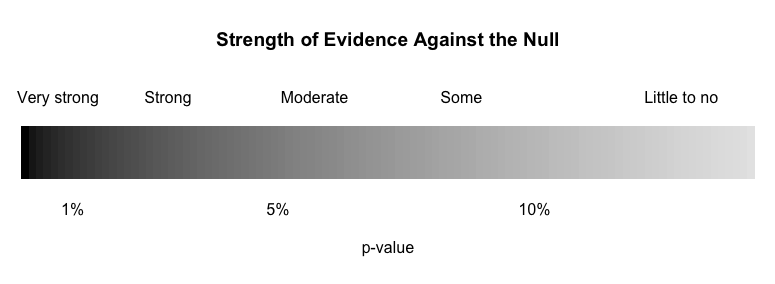
\includegraphics[width=0.9\linewidth]{images/soe_gradient_grayscale} \end{center}

\hypertarget{interpret-the-p-value}{%
\subsubsection*{Interpret the p-value}\label{interpret-the-p-value}}
\addcontentsline{toc}{subsubsection}{Interpret the p-value}

The p-value measures the probability that we observe a sample proportion as extreme as what was seen in the data or more extreme (matching the direction of the Ha) IF the null hypothesis is true.

\begin{enumerate}
\def\labelenumi{\arabic{enumi}.}
\setcounter{enumi}{9}
\tightlist
\item
  What did we assume to create the null distribution?
\end{enumerate}

\vspace{1in}

\begin{enumerate}
\def\labelenumi{\arabic{enumi}.}
\setcounter{enumi}{10}
\tightlist
\item
  What value did we compare to the null distribution to find the p-value?
\end{enumerate}

\vspace{0.3in}

\begin{enumerate}
\def\labelenumi{\arabic{enumi}.}
\setcounter{enumi}{11}
\item
  What direction did we count simulations from the statistic?
  \vspace{0.3in}
\item
  Fill in the blanks below to interpret the p-value.
\end{enumerate}

\setstretch{1.5}

We would observe a sample proportion of (value of the sample proportion )\hrulefill  

or (greater, less, more extreme) \hrulefill   

with a probability of (value of p-value) \hrulefill  

IF we assume (\(H_0\) in context) \hrulefill.

\setstretch{1}
\vspace{12pt}

\hypertarget{communicate-the-results-and-answer-the-research-question}{%
\subsubsection*{Communicate the results and answer the research question}\label{communicate-the-results-and-answer-the-research-question}}
\addcontentsline{toc}{subsubsection}{Communicate the results and answer the research question}

When we write a conclusion we answer the research question by stating how much evidence there is for the alternative hypothesis.

\begin{enumerate}
\def\labelenumi{\arabic{enumi}.}
\setcounter{enumi}{13}
\tightlist
\item
  Write a conclusion in context of the study. How much evidence does the data provide in support of the alternative hypothesis?
\end{enumerate}

\vspace{1in}

\hypertarget{take-home-messages-7}{%
\subsection{Take-home messages}\label{take-home-messages-7}}

\begin{enumerate}
\def\labelenumi{\arabic{enumi}.}
\item
  The null distribution is created based on the assumption the null hypothesis is true. We compare the sample statistic to the distribution to find the likelihood of observing this statistic.
\item
  The p-value measures the probability of observing the sample statistic or more extreme (in direction of the alternative hypothesis) is the null hypothesis is true.
\end{enumerate}

\hypertarget{additional-notes-7}{%
\subsection{Additional notes}\label{additional-notes-7}}

Use this space to summarize your thoughts and take additional notes on today's activity and material covered.

\newpage

\hypertarget{week-6-lab-helper-hinderer-simulation-based-confidence-interval}{%
\section{Week 6 Lab: Helper-Hinderer --- Simulation-based Confidence Interval}\label{week-6-lab-helper-hinderer-simulation-based-confidence-interval}}

\setstretch{1}

\hypertarget{learning-outcomes-9}{%
\subsection{Learning outcomes}\label{learning-outcomes-9}}

\begin{itemize}
\item
  Use bootstrapping to find a confidence interval for a single proportion.
\item
  Interpret a confidence interval for a single proportion.
\end{itemize}

\hypertarget{terminology-review-7}{%
\subsection{Terminology review}\label{terminology-review-7}}

In today's activity, we will introduce simulation-based confidence intervals for a single proportion. Some terms covered in this activity are:

\begin{itemize}
\item
  Parameter of interest
\item
  Bootstrapping
\item
  Confidence interval
\end{itemize}

To review these concepts, see Chapters 10 \& 14 in your textbook.

\hypertarget{helper-hinderer-2}{%
\subsection{Helper-Hinderer}\label{helper-hinderer-2}}

In the last class, we found very strong evidence that the true proportion of infants who will choose the helper character is greater than 0.5. But what \emph{is} the true proportion of infants who will choose the helper character? We will use this same study to estimate this parameter of interest by creating a confidence interval.

As a reminder: Do young children know the difference between helpful and unhelpful behavior? A study by Hamblin, Wynn, and Bloom reported in Nature (Hamblin, Wynn, and Bloom 2007) was intended to check young kids' feelings about helpful and non-helpful behavior. Non-verbal infants ages 6 to 10 months were shown short videos with different shapes either helping or hindering the climber. Researchers were hoping to assess: Are infants more likely to preferentially choose the helper toy over the hinderer toy? In the study, of the 16 infants age 6 to 10 months, 14 chose the \emph{helper} toy and 2 chose the \emph{hinderer} toy.

A \textbf{point estimate} (our observed statistic) provides a single plausible value for a parameter. However, a point estimate is rarely perfect; usually there is some error in the estimate. In addition to supplying a point estimate of a parameter, a next logical step would be to provide a plausible \emph{range} of values for the parameter. This plausible range of values for the population parameter is called an \textbf{interval estimate} or \textbf{confidence interval}.

\hypertarget{activity-intro}{%
\subsubsection*{Activity intro}\label{activity-intro}}
\addcontentsline{toc}{subsubsection}{Activity intro}

\begin{enumerate}
\def\labelenumi{\arabic{enumi}.}
\tightlist
\item
  What is the value of the point estimate?
\end{enumerate}

\vspace{0.3in}

\begin{enumerate}
\def\labelenumi{\arabic{enumi}.}
\setcounter{enumi}{1}
\tightlist
\item
  If we took another random sample of 16 infants, would we get the exact same point estimate? Explain why or why not.
\end{enumerate}

\vspace{0.5in}

In today's activity, we will use bootstrapping to find a 95\% confidence interval for \(\pi\), the parameter of interest.

\begin{enumerate}
\def\labelenumi{\arabic{enumi}.}
\setcounter{enumi}{2}
\tightlist
\item
  In your own words, explain the bootstrapping process.
  \vspace{0.5in}
\end{enumerate}

\hypertarget{use-statistical-analysis-methods-to-draw-inferences-from-the-data-1}{%
\subsubsection*{Use statistical analysis methods to draw inferences from the data}\label{use-statistical-analysis-methods-to-draw-inferences-from-the-data-1}}
\addcontentsline{toc}{subsubsection}{Use statistical analysis methods to draw inferences from the data}

\begin{enumerate}
\def\labelenumi{\arabic{enumi}.}
\setcounter{enumi}{3}
\tightlist
\item
  Write out the parameter of interest for this study in words. \emph{Hint: this is the same as in Activity 6A.}
\end{enumerate}

\vspace{0.5in}

To use the computer simulation to create a bootstrap distribution, we will need to enter the

\begin{itemize}
\tightlist
\item
  ``sample size'' (the number of observational units or cases in the sample),
\item
  ``number of successes'' (the number of cases that choose the helper character),
\item
  ``number of repetitions'' (the number of samples to be generated), and
\item
  the ``confidence level'' (which level of confidence are we using to create the confidence interval).
\end{itemize}

\begin{enumerate}
\def\labelenumi{\arabic{enumi}.}
\setcounter{enumi}{4}
\tightlist
\item
  What values should be entered for each of the following into the simulation to create the bootstrap distribution of sample proportions to find a 95\% confidence interval?
  \vspace{1mm}
\end{enumerate}

\begin{itemize}
\tightlist
\item
  Sample size:
\end{itemize}

\vspace{.1in}

\begin{itemize}
\tightlist
\item
  Number of successes:
\end{itemize}

\vspace{.1in}

\begin{itemize}
\tightlist
\item
  Number of repetitions:
\end{itemize}

\vspace{.1in}

\begin{itemize}
\tightlist
\item
  Confidence level (as a decimal):
\end{itemize}

\vspace{.1in}

We will use the \texttt{one\_proportion\_bootstrap\_CI()} function in R (in the \texttt{catstats} package) to simulate the bootstrap distribution of sample proportions and calculate a confidence interval. Using the provided R script file, fill in the values/words for each \texttt{xx} with your answers from question 5 in the one proportion bootstrap confidence interval (CI) code to create a bootstrap distribution with 1000 simulations. Then highlight and run lines 1--7.

\begin{Shaded}
\begin{Highlighting}[]
\FunctionTok{one\_proportion\_bootstrap\_CI}\NormalTok{(}\AttributeTok{sample\_size =}\NormalTok{ xx, }\CommentTok{\# Sample size}
                    \AttributeTok{number\_successes =}\NormalTok{ xx, }\CommentTok{\# Observed number of successes}
                    \AttributeTok{number\_repetitions =} \DecValTok{1000}\NormalTok{, }\CommentTok{\# Number of bootstrap samples to use}
                    \AttributeTok{confidence\_level =} \FloatTok{0.95}\NormalTok{) }\CommentTok{\# Confidence level as a decimal}
\end{Highlighting}
\end{Shaded}

\newpage

\begin{enumerate}
\def\labelenumi{\arabic{enumi}.}
\setcounter{enumi}{5}
\tightlist
\item
  Sketch the bootstrap distribution created below.
\end{enumerate}

\vspace{1.8in}

\begin{enumerate}
\def\labelenumi{\arabic{enumi}.}
\setcounter{enumi}{6}
\item
  What is the value at the center of this bootstrap distribution? Why does this make sense?
  \vspace{.8in}
\item
  \textbf{Explain why the two vertical lines are at the 2.5th percentile and the 97.5th percentile.}
\end{enumerate}

\vspace{.7in}

\begin{enumerate}
\def\labelenumi{\arabic{enumi}.}
\setcounter{enumi}{8}
\tightlist
\item
  Report the 95\% bootstrapped confidence interval for \(\pi\). Use interval notation: (lower value, upper value).
\end{enumerate}

\vspace{0.2in}

\begin{enumerate}
\def\labelenumi{\arabic{enumi}.}
\setcounter{enumi}{9}
\tightlist
\item
  \textbf{Interpret the 95\% confidence interval in context.}
\end{enumerate}

\vspace{.7in}

\hypertarget{communicate-the-results-and-answer-the-research-question-1}{%
\subsubsection*{Communicate the results and answer the research question}\label{communicate-the-results-and-answer-the-research-question-1}}
\addcontentsline{toc}{subsubsection}{Communicate the results and answer the research question}

\begin{enumerate}
\def\labelenumi{\arabic{enumi}.}
\setcounter{enumi}{10}
\tightlist
\item
  \textbf{Is the value 0.5 (the null value) in the 95\% confidence interval?}
\end{enumerate}

\vspace{.2in}

~~~\textbf{Explain how this indicates that the p-value provides strong evidence against the null.}

\newpage

\hypertarget{effect-of-confidence-level}{%
\subsubsection*{Effect of confidence level}\label{effect-of-confidence-level}}
\addcontentsline{toc}{subsubsection}{Effect of confidence level}

\begin{enumerate}
\def\labelenumi{\arabic{enumi}.}
\setcounter{enumi}{11}
\tightlist
\item
  Suppose instead of finding a 95\% confidence interval, we found a 90\% confidence interval. Would you expect the 90\% confidence interval to be narrower or wider? Explain your answer.
\end{enumerate}

\vspace{0.4in}

\begin{enumerate}
\def\labelenumi{\arabic{enumi}.}
\setcounter{enumi}{12}
\tightlist
\item
  The following R code produced the bootstrap distribution with 1000 simulations that follows. Circle the value that changed in the code.
\end{enumerate}

\begin{Shaded}
\begin{Highlighting}[]
\FunctionTok{one\_proportion\_bootstrap\_CI}\NormalTok{(}\AttributeTok{sample\_size =} \DecValTok{16}\NormalTok{, }\CommentTok{\# Sample size}
                    \AttributeTok{number\_successes =} \DecValTok{14}\NormalTok{, }\CommentTok{\# Observed number of successes}
                    \AttributeTok{number\_repetitions =} \DecValTok{1000}\NormalTok{, }\CommentTok{\# Number of bootstrap samples to use}
                    \AttributeTok{confidence\_level =} \FloatTok{0.90}\NormalTok{) }\CommentTok{\# Confidence level as a decimal}
\end{Highlighting}
\end{Shaded}

\begin{center}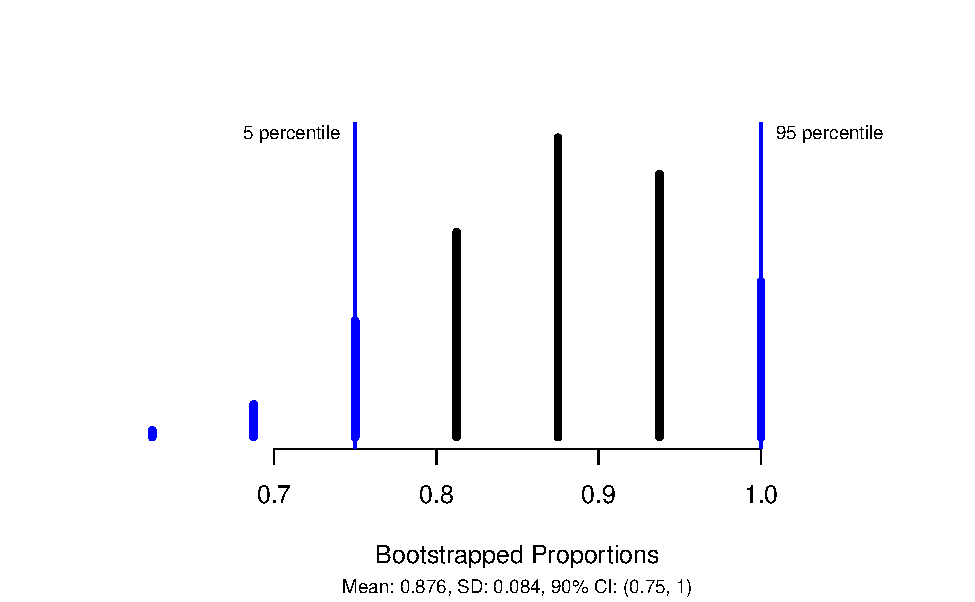
\includegraphics[width=0.7\linewidth]{06-L04-inference-1cat_CI-simulation_files/figure-latex/unnamed-chunk-2-1} \end{center}

\begin{enumerate}
\def\labelenumi{\arabic{enumi}.}
\setcounter{enumi}{13}
\tightlist
\item
  Report both the 95\% confidence interval (question 9) and the 90\% confidence interval (question 13). Is the 90\% confidence interval narrower or wider than the 95\% confidence interval?
\end{enumerate}

\vspace{0.5in}

\begin{enumerate}
\def\labelenumi{\arabic{enumi}.}
\setcounter{enumi}{14}
\tightlist
\item
  Explain why the upper value of the confidence interval is truncated at 1.
\end{enumerate}

\vspace{0.5in}

\newpage

\setstretch{1.5}

\begin{enumerate}
\def\labelenumi{\arabic{enumi}.}
\setcounter{enumi}{15}
\tightlist
\item
  Fill in the blanks below to write a paragraph summarizing the results of the study as if writing a press release. \textbf{Complete your group's paragraph on Gradescope.}\\
  Researchers were interested if infants observe social cues and would be more likely to choose the helper toy over the hinderer toy. In a sample of (sample size) \_\_\_\_\_\_\_\_\_\_\_\_\_infants, (number of successes) \_\_\_\_\_\_\_\_\_\_\_\_\_\_\_chose the helper toy. A simulation null distribution with 1000 simulations was created in RStudio. The p-value was found by calculating the proportion of simulations in the null distribution at the sample statistic of 0.875 and greater. This resulted in a p-value of (value of p-value)\_\_\_\_\_\_\_\_\_\_\_\_\_\_\_. We would observe a sample proportion of (value of the sample proportion) \_\_\_\_\_\_\_\_\_\_\_\_\_\_\_\_\_\_\_\_\_\_ or (greater, less, more extreme) \_\_\_\_\_\_\_\_\_\_\_\_\_\_\_\_\_\_\_\_\_ with a probability of (value of p-value)\_\_\_\_\_\_\_\_\_\_\_\_\_\_\_\_\_\_\_\\
  IF we assume (\(H_0\) in context) \_\_\_\_\_\_\_\_\_\_\_\_\_\_\_\_\_\_\_\_\_\_\_\_\_\_\_\_\_\_\_\_\_\_\_\_\_\_\_\_\_\_\_\_.
  Based on this p-value, there is (very strong/little to no) \_\_\_\_\_\_\_\_\_\_\_\_\_\_\_\_\_\_\_\_\_\_ evidence that the (sample/true)\_\_\_\_\_\_\_\_\_\_\_\_\_\_\_\_\_\_\_\_\_ proportion of infants age 6 to 10 months who will choose the helper toy is (greater than, less than, not equal to) \_\_\_\_\_\_\_\_\_\_\_\_\_\_\_\_\_\_\_\_\_ 0.5. In addition, a 95\% confidence interval was found for the parameter of interest. We are 95\% confident that the (true/sample)\_\_\_\_\_\_\_\_\_\_\_\_\_\_\_\_\_\_\_\_\_\_\_\_\_ proportion of infants age 6 to 10 months who will choose the helper toy is between (lower value)\_\_\_\_\_\_\_\_\_\_\_\_\_\_\_\_ and (upper value)\_\_\_\_\_\_\_\_\_\_\_\_\_\_\_\_\_\_\_\_. The results of this study can be generalized to (all infants age 6 to 10 months/infants similar to those in this study)\_\_\_\_\_\_\_\_\_\_\_\_\_\_\_\_\_\_\_\_\_\_\_\_\_\_\_ as the researchers (did/did not)\_\_\_\_\_\_\_\_\_\_\_\_\_\_\_\_\_\_\_\_\_ select a random sample.
\end{enumerate}

\setstretch{1}

\hypertarget{take-home-messages-8}{%
\subsection{Take-home messages}\label{take-home-messages-8}}

\begin{enumerate}
\def\labelenumi{\arabic{enumi}.}
\item
  The goal in a hypothesis test is to assess the strength of evidence for an effect, while the goal in creating a confidence interval is to determine how large the effect is. A \textbf{confidence interval} is a range of \emph{plausible} values for the parameter of interest.
\item
  A confidence interval is built around the point estimate or observed calculated statistic from the sample. This means that the sample statistic is always the center of the confidence interval. A confidence interval includes a measure of sample to sample variability represented by the \textbf{margin of error}.
\item
  In simulation-based methods (bootstrapping), a simulated distribution of possible sample statistics is created showing the possible sample-to-sample variability. Then we find the middle \(X\) percent of the distribution around the sample statistic using the percentile method to give the range of values for the confidence interval. This shows us that we are \(X\)\% confident that the parameter is within this range, where \(X\) represents the level of confidence.
\item
  When the null value is within the confidence interval, it is a plausible value for the parameter of interest; thus, we would find a larger p-value for a hypothesis test of that null value. Conversely, if the null value is NOT within the confidence interval, we would find a small p-value for the hypothesis test and strong evidence against this null hypothesis.
\item
  To create one simulated sample on the bootstrap distribution for a sample proportion, label \(n\) cards with the original responses. Draw with replacement \(n\) times. Calculate and plot the resampled proportion of successes.
\end{enumerate}

\hypertarget{additional-notes-8}{%
\subsection{Additional notes}\label{additional-notes-8}}

Use this space to summarize your thoughts and take additional notes on today's activity and material covered.

\newpage

\hypertarget{out-of-class-activity-7-handedness-of-male-boxers}{%
\section{Out of Class Activity 7: Handedness of Male Boxers}\label{out-of-class-activity-7-handedness-of-male-boxers}}

\setstretch{1}

\hypertarget{learning-outcomes-10}{%
\subsection{Learning outcomes}\label{learning-outcomes-10}}

\begin{itemize}
\item
  Describe and perform a theory-based hypothesis test for a single proportion.
\item
  Check the appropriate conditions to use a theory-based hypothesis test.
\item
  Calculate and interpret the standardized sample proportion.
\item
  Interpret and evaluate a p-value for a theory-based hypothesis test for a single proportion.
\item
  Use the normal distribution to find the p-value.
\end{itemize}

\hypertarget{terminology-review-8}{%
\subsection{Terminology review}\label{terminology-review-8}}

In this activity, we will introduce theory-based hypothesis tests for a single categorical variable. Some terms covered in this activity are:

\begin{itemize}
\item
  Parameter of interest
\item
  Standardized Statistic
\item
  Normal distribution
\item
  p-value
\end{itemize}

To review these concepts, see Chapter 11 \& 14 in your textbook.

Activities 6A, 6B, and the Week 6 Lab covered simulation-based methods for hypothesis tests involving a single categorical variable. This activity covers theory-based methods for testing a single categorical variable.

\hypertarget{handedness-of-male-boxers}{%
\subsection{Handedness of male boxers}\label{handedness-of-male-boxers}}

Left-handedness is a trait that is found in about 10\% of the general population. Past studies have shown that left-handed men are over-represented among professional boxers (Richardson and Gilman 2019). The fighting claim states that left-handed men have an advantage in competition. In this random sample of 500 male professional boxers, we want to see if there is an over-prevalence of left-handed fighters. In the sample of 500 male boxers, 81 were left-handed.

\begin{Shaded}
\begin{Highlighting}[]
 \CommentTok{\# Read in data set}
\NormalTok{boxers }\OtherTok{\textless{}{-}} \FunctionTok{read.csv}\NormalTok{(}\StringTok{"https://math.montana.edu/courses/s216/data/Male\_boxers\_sample.csv"}\NormalTok{)}
\NormalTok{boxers }\SpecialCharTok{\%\textgreater{}\%} \FunctionTok{count}\NormalTok{(Stance)  }\CommentTok{\# Count number in each Stance category}
\end{Highlighting}
\end{Shaded}

\begin{verbatim}
#>         Stance   n
#> 1  left-handed  81
#> 2 right-handed 419
\end{verbatim}

\hypertarget{review-of-summary-statistics}{%
\subsection*{Review of summary statistics}\label{review-of-summary-statistics}}
\addcontentsline{toc}{subsection}{Review of summary statistics}

\begin{enumerate}
\def\labelenumi{\arabic{enumi}.}
\tightlist
\item
  Write out the parameter of interest for this study.
\end{enumerate}

\vspace{0.8in}

\begin{enumerate}
\def\labelenumi{\arabic{enumi}.}
\setcounter{enumi}{1}
\item
  Write out the null hypothesis in words.
  \vspace{0.8in}
\item
  Write out the alternative hypothesis in notation.
  \vspace{0.3in}
\item
  Give the value of the summary statistic (sample proportion) for this study. Use proper notation.
\end{enumerate}

\vspace{0.3in}

\hypertarget{theory-based-methods}{%
\subsection*{Theory-based methods}\label{theory-based-methods}}
\addcontentsline{toc}{subsection}{Theory-based methods}

The sampling distribution of a single proportion --- how that proportion varies from sample to sample --- can be mathematically modeled using the normal distribution if certain conditions are met.

Conditions for the sampling distribution of \(\hat{p}\) to follow an approximate normal distribution:

\begin{itemize}
\item
  \textbf{Independence}: The sample's observations are independent, e.g., are from a simple random sample. (\emph{Remember}: This also must be true to use simulation methods!)
\item
  \textbf{Success-failure condition}: We \emph{expect} to see at least 10 successes and 10 failures in the sample, \(n\hat{p}≥10\) and \(n(1-\hat{p})≥10\).
\end{itemize}

\begin{enumerate}
\def\labelenumi{\arabic{enumi}.}
\setcounter{enumi}{4}
\tightlist
\item
  Verify that the independence condition is satisfied.
\end{enumerate}

\vspace{0.5in}

\begin{enumerate}
\def\labelenumi{\arabic{enumi}.}
\setcounter{enumi}{5}
\tightlist
\item
  Is the success-failure condition met to model the data with the normal distribution? Show your work to support your answer.
\end{enumerate}

\vspace{1in}
\newpage

To calculate the standardized statistic we use the general formula

\[
Z = \frac{\text{point estimate} - \text{null value}}{SE_0(\text{point estimate})}.
\]
For a single categorical variable the standardized sample proportion is calculated using

\[
Z = \frac{\hat{p} - \pi_0}{SE_0(\hat{p})},
\]
where the standard error is calculated using the null value:

\[SE_0(\hat{p})=\sqrt{\frac{\pi_0(1-\pi_0)}{n}}\].

The standard error of the sample proportion measures the variability of possible sample proportions from the actual proportion. In other words, how far each possible sample proportion is from the actual proportion on average. For this study, the null standard error of the sample proportion is calculated using the null value, 0.1.

\[SE_0(\hat{p})=\sqrt{\frac{0.1(1-0.1)}{500}} = 0.013\].

Each sample proportion of male boxers that are left-handed is 0.013 from the true proportion of male boxers that are left-handed, on average.

\begin{enumerate}
\def\labelenumi{\arabic{enumi}.}
\setcounter{enumi}{6}
\tightlist
\item
  Using the null standard error of the sample proportion, calculate the standardized sample proportion.
\end{enumerate}

\vspace{0.6in}

The standardized statistic is used as a ruler to measure how far the sample statistic is from the null value. Essentially, we are converting the sample proportion into a measure of standard errors to compare to the standard normal distribution.

\begin{enumerate}
\def\labelenumi{\arabic{enumi}.}
\setcounter{enumi}{7}
\tightlist
\item
  Using the 68-95-99.7 rule in Section 5.2.5 to guide you, fill in the percentages on the standard normal distribution displayed in Figure \ref{fig:simpleNormalcurve}, and also mark the value of the standardized statistic calculated in question 8.
\end{enumerate}

\begin{figure}

{\centering 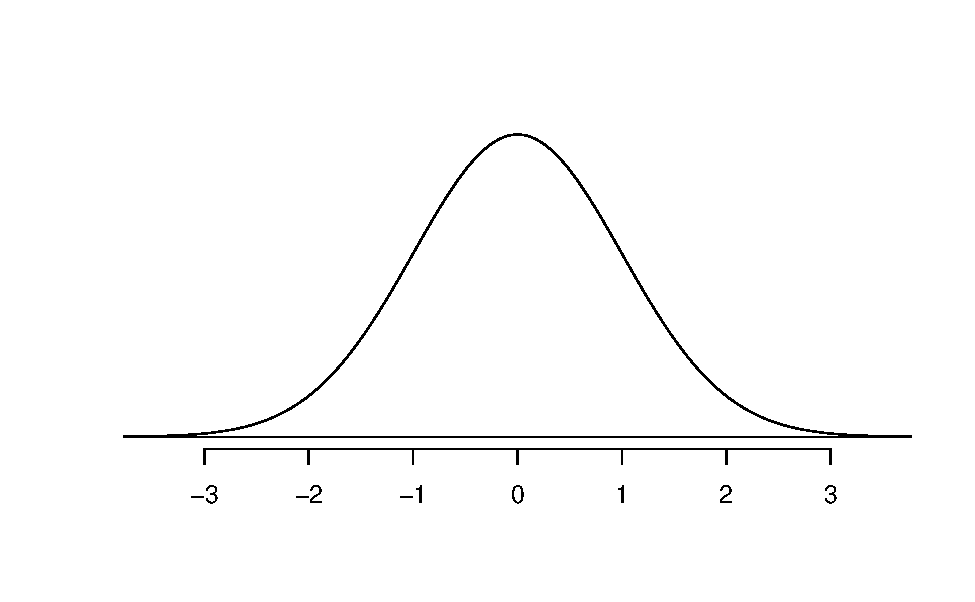
\includegraphics[width=0.5\linewidth]{07-OCA05-inference-1cat_test-theory_files/figure-latex/simpleNormalcurve-1} 

}

\caption{A standard normal curve.}\label{fig:simpleNormalcurve}
\end{figure}

\newpage

The standardized statistic measures the \emph{number of standard errors the sample statistic is from the null value}.

\begin{enumerate}
\def\labelenumi{\arabic{enumi}.}
\setcounter{enumi}{8}
\tightlist
\item
  Interpret the standardized sample proportion from question 7 in context of the problem.
\end{enumerate}

\vspace{.8in}

We will use the \texttt{pnorm()} function in \texttt{R} to find the p-value. Use the provided \texttt{R} script file and enter the value of the standardized statistic calculated in question 7 at \texttt{xx} in line 7; highlight and run lines 7--9. Notice that in line 9 it says \texttt{lower.tail\ =\ FALSE}. \texttt{R} will calculate the p-value \emph{greater} than the value of the standardized statistic.

Notes:

\begin{itemize}
\tightlist
\item
  Use \texttt{lower.tail\ =\ TRUE} when doing a left-sided test.
\item
  Use \texttt{lower.tail\ =\ FALSE} when doing a right-sided test.
\item
  To find a two-sided p-value, use a left-sided test for negative Z or a right-sided test for positive Z, then multiply the value found by 2 to get the p-value.
\end{itemize}

\begin{Shaded}
\begin{Highlighting}[]
\FunctionTok{pnorm}\NormalTok{(xx, }\CommentTok{\# Enter value of standardized statistic}
      \AttributeTok{m=}\DecValTok{0}\NormalTok{, }\AttributeTok{s=}\DecValTok{1}\NormalTok{, }\CommentTok{\# Using the standard normal mean = 0, sd = 1}
      \AttributeTok{lower.tail=}\ConstantTok{FALSE}\NormalTok{) }\CommentTok{\# Gives a p{-}value greater than the standardized statistic}
\end{Highlighting}
\end{Shaded}

\begin{enumerate}
\def\labelenumi{\arabic{enumi}.}
\setcounter{enumi}{9}
\item
  Report the p-value obtained from the \texttt{R} output.
  \vspace{0.3in}
\item
  Write a conclusion based on the value of the p-value.
  \newpage
\end{enumerate}

\hypertarget{take-home-messages-9}{%
\subsection{Take-home messages}\label{take-home-messages-9}}

\begin{enumerate}
\def\labelenumi{\arabic{enumi}.}
\item
  Both simulation and theory-based methods can be used to find a p-value for a hypothesis test. In order to use theory-based methods we need to check that both the independence and the success-failure conditions are met.
\item
  The standardized statistic measures how many standard errors the statistic is from the null value. The larger the standardized statistic the more evidence there is against the null hypothesis.
\end{enumerate}

\newpage

\hypertarget{additional-notes-9}{%
\subsection{Additional notes}\label{additional-notes-9}}

Use this space to summarize your thoughts and take additional notes on today's activity and material covered.

\newpage

\hypertarget{activity-7-handedness-of-male-boxers-theory-ci}{%
\section{Activity 7: Handedness of Male Boxers --- Theory CI}\label{activity-7-handedness-of-male-boxers-theory-ci}}

\setstretch{1}

\hypertarget{learning-objectives}{%
\subsection{Learning objectives}\label{learning-objectives}}

\begin{itemize}
\item
  Calculate a theory-based confidence interval for a single proportion.
\item
  Check the appropriate conditions to find a theory-based confidence interval.
\item
  Interpret a confidence interval for a single proportion.
\item
  Use the normal distribution to find the multiplier needed for a confidence interval
\end{itemize}

\hypertarget{terminology-review-9}{%
\subsection{Terminology review}\label{terminology-review-9}}

In this activity, we will introduce theory-based confidence intervals for a single proportion. Some terms covered in this activity are:

\begin{itemize}
\item
  Parameter of interest
\item
  Multiplier
\item
  Normal distribution
\end{itemize}

To review these concepts, see Chapters 11 \& 14 in your textbook.

\hypertarget{handedness-of-male-boxers-1}{%
\subsection{Handedness of Male Boxers}\label{handedness-of-male-boxers-1}}

In the out of class activity we found very strong evidence that the true proportion of male boxers that are left-handed is greater than 0.1. In this activity we will use the same data set to find the theory-based 95\% confidence interval.

Remember from the last activity: Left-handedness is a trait that is found in about 10\% of the general population. Past studies have shown that left-handed men are over-represented among professional boxers. The fighting claim states that left-handed men have an advantage in competition. In this random sample of 500 male professional boxers, we want to see if there is an over-prevalence of left-handed fighters. In the sample of 500 male boxers, 81 were left-handed.

Recall that to use theory-based methods we must check the conditions to approximate the sampling distribution with the normal distribution. From the previous activity, we saw that independence was satisfied as the researchers took a random sample and that the sample had more than 10 successes and 10 failures.

\newpage

\hypertarget{theory-based-confidence-interval}{%
\subsubsection*{Theory-based confidence interval}\label{theory-based-confidence-interval}}
\addcontentsline{toc}{subsubsection}{Theory-based confidence interval}

To calculate a theory-based 95\% confidence interval for \(\pi\), we will first find the \textbf{standard error} of \(\hat{p}\) by plugging in the value of \(\hat{p}\) for \(\pi\) in \(SD(\hat{p})\):

\[SE(\hat{p}) = \sqrt{\frac{\hat{p}(1-\hat{p})}{n}}.\]
Note that we do not include a ``0'' subscript, since we are not assuming a null hypothesis.

\begin{enumerate}
\def\labelenumi{\arabic{enumi}.}
\tightlist
\item
  Calculate the standard error of the sample proportion to find a 95\% confidence interval.
\end{enumerate}

\vspace{0.5in}

To find the confidence interval, we will add and subtract the \textbf{margin of error} to the point estimate:

\[\text{point estimate}\pm\text{margin of error}\]
\[\hat{p}\pm z^* SE(\hat{p})\]
\[ME = z^* SE(\hat{p})\]

The \(z^*\) multiplier is the percentile of a standard normal distribution that corresponds to our confidence level. If our confidence level is 95\%, we find the Z values that encompass the middle 95\% of the standard normal distribution. If 95\% of the standard normal distribution should be in the middle, that leaves 5\% in the tails, or 2.5\% in each tail.

\begin{enumerate}
\def\labelenumi{\arabic{enumi}.}
\setcounter{enumi}{1}
\tightlist
\item
  Fill in the normal distribution shown in figure 7.2 to show how R found the \(z^*\) multiplier.
\end{enumerate}

\begin{figure}

{\centering 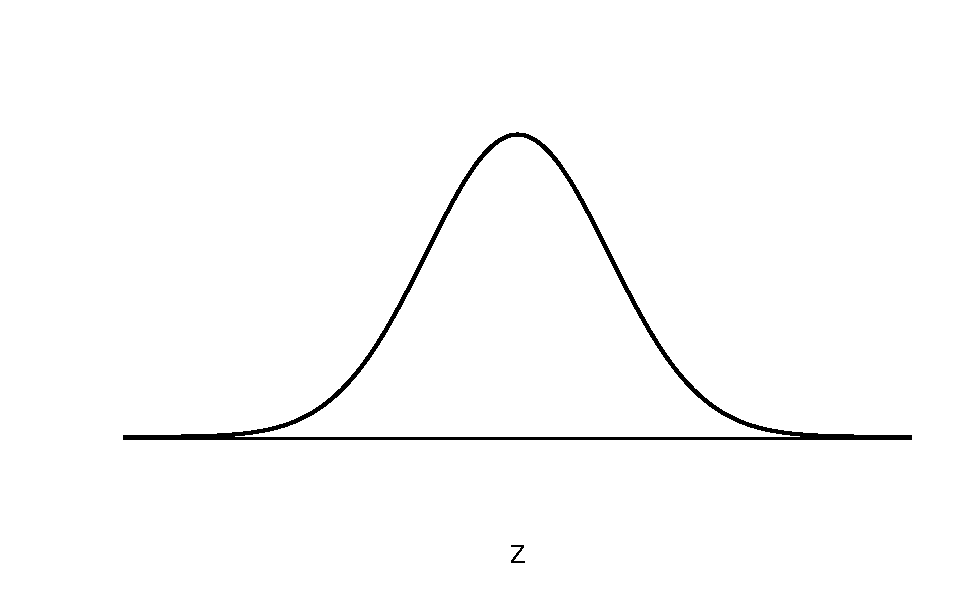
\includegraphics[width=0.5\linewidth]{07-A06-inference-1cat_CI-theory_files/figure-latex/simpleNormaldist-1} 

}

\caption{A standard normal curve.}\label{fig:simpleNormaldist}
\end{figure}

The \texttt{qnorm()} function in R will tell us the \(z^*\) value for the desired percentile (in this case, 95\% + 2.5\% = 97.5\% percentile). Enter the value of 0.975 for xx in the provided R script file. This will give the value of the multiplier for a 95\% confidence interval.

\begin{Shaded}
\begin{Highlighting}[]
\FunctionTok{qnorm}\NormalTok{(xx) }\CommentTok{\# Multiplier for 95\% confidence interval}
\end{Highlighting}
\end{Shaded}

\begin{enumerate}
\def\labelenumi{\arabic{enumi}.}
\setcounter{enumi}{2}
\item
  Report the value of the multiplier needed to calculate the 95\% confidence interval for the true proportion of male boxers that are left-handed?
  \vspace{0.3in}
\item
  Calculate the margin of error for the 95\% confidence interval.
  \vspace{1in}
\item
  Calculate the 95\% confidence interval for the parameter of interest.
  \vspace{0.5in}
\item
  Interpret the 95\% confidence interval in the context of the problem.
  \vspace{1in}
\item
  Is the null value, 0.1, contained in the 95\% confidence interval? Explain, based on the p-value from the last activity, why you expected this to be true.
  \vspace{0.5in}
\end{enumerate}

\hypertarget{simulation-methods}{%
\subsubsection*{Simulation Methods}\label{simulation-methods}}
\addcontentsline{toc}{subsubsection}{Simulation Methods}

In activity 7A, we found that the success-failure condition was met to use theory-based methods. Here we will use simulation methods to find a 95\% confidence interval for the parameter of interest.

Use the \texttt{one\_proportion\_bootstrap\_CI()} function in R to simulate the bootstrap distribution of sample proportions and calculate a confidence interval. Using the provided R script file, fill in the values/words for each \texttt{xx} in the one proportion bootstrap confidence interval (CI) code to create a bootstrap distribution with 1000 simulations. Make sure to run the library(catstats) function before running the one\_proportion\_bootstrap\_CI function.

\begin{Shaded}
\begin{Highlighting}[]
\FunctionTok{one\_proportion\_bootstrap\_CI}\NormalTok{(}\AttributeTok{sample\_size =}\NormalTok{ xx, }\CommentTok{\# Sample size}
                    \AttributeTok{number\_successes =}\NormalTok{ xx, }\CommentTok{\# Observed number of successes}
                    \AttributeTok{number\_repetitions =} \DecValTok{1000}\NormalTok{, }\CommentTok{\# Number of bootstrap samples to use}
                    \AttributeTok{confidence\_level =} \FloatTok{0.95}\NormalTok{) }\CommentTok{\# Confidence level as a decimal}
\end{Highlighting}
\end{Shaded}

\begin{enumerate}
\def\labelenumi{\arabic{enumi}.}
\setcounter{enumi}{7}
\tightlist
\item
  Report the simulation 95\% confidence interval. Is this confidence interval similar to the confidence interval calculated in question 5? Explain why this makes sense.
\end{enumerate}

\vspace{0.8in}

\hypertarget{what-does-confidence-mean}{%
\subsection*{\texorpdfstring{What does \emph{confidence} mean?}{What does confidence mean?}}\label{what-does-confidence-mean}}
\addcontentsline{toc}{subsection}{What does \emph{confidence} mean?}

In the interpretation of a 95\% confidence interval, we say that we are 95\% confident that the parameter is within the confidence interval. Why are we able to make that claim? What does it mean to say ``we are 95\% confident''?

For this part of the activity we will assume that the the true proportion of male boxers that are left-handed is 0.1. \emph{Note: we are making assumptions about the population here. This is not based on our calculated data, but we will use this applet to better understand what happens when we take many, many samples from this believed population.}

\begin{enumerate}
\def\labelenumi{\arabic{enumi}.}
\setcounter{enumi}{8}
\item
  Go to this website, \url{http://www.rossmanchance.com/ISIapplets.html} and choose `Simulating Confidence Intervals'. In the input on the left-hand side of the screen enter 0.1 for \(\pi\) (the true value), 500 for \(n\), and 100 for `Number of intervals'. Click `sample'.
  \vspace{1mm}

  \begin{enumerate}
  \def\labelenumii{\alph{enumii}.}
  \item
    In the graph on the bottom right, click on a green dot. Write down the confidence interval for this sample given on the graph on the left. Does this confidence interval contain the true value of 0.1?
    \vspace{0.5in}
  \item
    Now click on a red dot. Write down the confidence interval for this sample. Does this confidence interval contain the true value of 0.1?
    \vspace{0.5in}
  \item
    How many intervals out of 100 contain \(\pi\), the true value of 0.1? \emph{Hint}: This is given to the left of the graph of green and red intervals.
    \vspace{0.5in}
  \end{enumerate}
\item
  Click on `sample' nine more times. Write down the `Running Total' for the proportion of intervals that contain \(\pi\).
\end{enumerate}

\vspace{0.5in}

\begin{enumerate}
\def\labelenumi{\arabic{enumi}.}
\setcounter{enumi}{10}
\tightlist
\item
  \textbf{Interpret the level of confidence. \emph{Hint}: What proportion of samples would we expect to give a confidence interval that contains the parameter of interest?}
\end{enumerate}

\vspace{0.8in}

\hypertarget{take-home-messages-10}{%
\subsection{Take-home messages}\label{take-home-messages-10}}

\begin{enumerate}
\def\labelenumi{\arabic{enumi}.}
\item
  In theory-based methods, we add and subtract a margin of error to the sample statistic. The margin of error is calculated using a multiplier that corresponds to the level of confidence times the variability (standard error) of the statistic.
\item
  The confidence interval calculated using theory-based methods should be similar to the confidence interval found using simulation methods provided the success-failure condition is met.
\end{enumerate}

\begin{enumerate}
\def\labelenumi{\arabic{enumi}.}
\setcounter{enumi}{2}
\tightlist
\item
  If repeat samples of the same size are selected from the population, approximately 95\% of samples will create a 95\% confidence interval that contains the parameter of interest.
\end{enumerate}

\hypertarget{additional-notes-10}{%
\subsection{Additional notes}\label{additional-notes-10}}

Use this space to summarize your thoughts and take additional notes on today's activity and material covered.

\newpage

\hypertarget{week-7-lab-errors-and-power}{%
\section{Week 7 Lab: Errors and Power}\label{week-7-lab-errors-and-power}}

\setstretch{1}

\hypertarget{learning-outcomes-11}{%
\subsection{Learning outcomes}\label{learning-outcomes-11}}

\begin{itemize}
\item
  Explain type 1 and type 2 errors in the context of a study.
\item
  Explain the power of a test in the context of a study.
\item
  Understand how changes in sample size, significance level, and the difference between the null value and the parameter value impact the power of a test.
\item
  Understand how significance level impacts the probability of a type 1 error.
\item
  Understand the relationship between the probability of a type 2 error and power.
\item
  Be able to distinguish between practical importance and statistical significance.
\end{itemize}

\hypertarget{terminology-review-10}{%
\subsection{Terminology review}\label{terminology-review-10}}

In this activity, we will examine the possible errors that can be made based on the decision in a hypothesis test as well as factors influencing the power of the test. Some terms covered in this activity are:

\begin{itemize}
\item
  Significance level
\item
  Type 1 error
\item
  Type 2 error
\item
  Power
\end{itemize}

To review these concepts, see Chapter 12 in the textbook.

\hypertarget{acl-recovery}{%
\subsection{ACL recovery}\label{acl-recovery}}

It is widely reported that the median recovery time for athletes who undergo surgery to repair a torn anterior cruciate ligament (ACL) is 8 months, indicating that 50\% of athletes return to their sport within 8 months after an ACL surgery. Suppose a local physical therapy company hopes to advertise that their rehabilitation program can increase this percentage.

\begin{enumerate}
\def\labelenumi{\arabic{enumi}.}
\item
  Write the parameter of interest (\(\pi\)) in words, in the context of this problem.
  \vspace{0.5in}
\item
  \textbf{Use proper notation to write the null and alternative hypothesis the company would need to test in order to check their advertisement claim.}
  \vspace{0.5in}
\end{enumerate}

After determining hypotheses and prior to collecting data, researchers should set a \textbf{significance level} for a hypothesis test. The significance level, represented by \(\alpha\) and most commonly 0.01, 0.05, or 0.10, is a cut-off for determining whether a p-value is small or not. The \emph{smaller} the p-value, the \emph{stronger} the evidence against the null hypothesis, so a p-value that is smaller than or equal to the significance level is strong enough evidence to \emph{reject the null hypothesis}. Similarly, the \emph{larger} the p-value, the \emph{weaker} the evidence against the null hypothesis, so a p-value that is larger than the significance level does not provide enough evidence against the null hypothesis and the researcher would \emph{fail to reject the null hypothesis}. Rejecting the null hypothesis or failing to reject the null hypothesis are the two \textbf{decisions} that can be made based on the data collected.

As you have already learned in this course, sample size of a study is extremely important. Often times, researchers will conduct what is called a power analysis to determine the appropriate sample size based on the goals of their research, including a desired \textbf{power} of their test. Power is the probability of correctly rejecting the null hypothesis, or the probability of the data providing strong evidence against the null hypothesis \emph{when the null hypothesis is false}.

The remainder of this lab will be spent investigating how different factors influence the power of a test, after which you will complete a power analysis for this physical therapy company.

\begin{itemize}
\item
  Navigate to \url{https://istats.shinyapps.io/power/}. \emph{Please note that this applet uses \(p_0\) to represent the null value rather than \(\pi_0\).}
\item
  Use the scale under ``Null Hypothesis value \(p_0\)'' to change the value to your null value from question 2.
\item
  Change the ``Alternative Hypothesis'' to the direction you wrote in question 2.
\item
  Leave all boxes un-checked. Do not change the scales under ``True value of \(p_0\)'', ``Sample size n'', or ``Type I Error \(\alpha\)''
\end{itemize}

The red distribution you see is the scaled-Normal distribution representing the null distribution for this hypothesis test, if the sample size was 50 and the significance level was 0.05. This means the red distribution is showing the probability of each possible sample proportion of athletes who returned to their sport within 8 months (\(\hat{p}\)) if we assume the null hypothesis is true.

\begin{enumerate}
\def\labelenumi{\arabic{enumi}.}
\setcounter{enumi}{2}
\item
  Based off this distribution and your alternative hypothesis, give one possible sample proportion which you think would lead to rejecting the null hypothesis. Explain how you decided on your value.
  \vspace{0.25in}
\item
  Check the box for ``Show Critical Value(s) and Rejection Region(s)''. You will now see a vertical line on the plot indicating the \emph{minimum} sample proportion which would lead to reject the null hypothesis. What is this value?\\
  \vspace{0.25in}
\item
  Notice that there are some sample proportions under the red line (when the null hypothesis is true) which would lead us to reject the null hypothesis. Give the range of sample proportions which would lead to rejecting the null hypothesis when the null hypothesis is true? What is the statistical name for this mistake?
  \vspace{0.4in}
\end{enumerate}

Check the ``Type I Error'' box under \textbf{Display}. This should verify (or correct) your answer to question 5! The area shaded in red represents the probability of making a \textbf{type 1 error} in our hypothesis test. Recall that a type 1 error is when we reject the null hypothesis even though the null hypothesis is true. To reject the null hypothesis, the p-value, which was found assuming the null hypothesis is true, must be less than or equal to the significance level. Therefore the significance level is the maximum probability of rejecting the null hypothesis when the null hypothesis is true, so the significance level IS the probability of making a type 1 error in a hypothesis test!

\begin{enumerate}
\def\labelenumi{\arabic{enumi}.}
\setcounter{enumi}{5}
\tightlist
\item
  \textbf{Based on the current applet settings, What percent of the null distribution is shaded red (what is the probability of making a type 1 error)?}
  \vspace{0.25in}
\end{enumerate}

Let's say this physical therapist company believes their program can get 70\% of athletes back to their sport within 8 months of an ACL surgery. In the applet, set the scale under ``True value of \(p\)'' to 0.7.

\begin{enumerate}
\def\labelenumi{\arabic{enumi}.}
\setcounter{enumi}{6}
\tightlist
\item
  Where is the blue distribution centered?
  \vspace{0.25in}
\end{enumerate}

The blue distribution that appears represents what the company believes, that 0.7 (not 0.5) is the true proportion of its clients who return to their sport within 8 months of ACL surgery. This blue distribution represents the idea that the \textbf{null hypothesis is false}.

\begin{enumerate}
\def\labelenumi{\arabic{enumi}.}
\setcounter{enumi}{7}
\tightlist
\item
  Consider the definition of power provided earlier in this lab. Do you believe the power of the test will be an area within the blue distribution or red distribution? How do you know? What about the probability of making a type 2 error?
  \vspace{1in}
\end{enumerate}

\begin{itemize}
\tightlist
\item
  Check the ``Type II Error'' and ``Power'' boxes under \textbf{Display}. This should verify (or correct) your answers to question 8! The area shaded in blue represents the probability of making a \textbf{type 2 error} in our hypothesis test (failing to reject the null hypothesis even though the null hypothesis is false). The area shaded in green represents the power of the test. Notice that the type 1 and type 2 errors rates and the power of the test are provided above the distribution.
\end{itemize}

\begin{enumerate}
\def\labelenumi{\arabic{enumi}.}
\setcounter{enumi}{8}
\tightlist
\item
  \textbf{Complete the following equation: Power + Type 2 Error Rate = . Explain why that equation makes sense.} \emph{Hint: Consider what power and type 2 error are conditional on.}
  \vspace{0.8in}
\end{enumerate}

Now let's investigate how changes in different factors influence the power of a test.

\begin{enumerate}
\def\labelenumi{\arabic{enumi}.}
\setcounter{enumi}{9}
\item
  Using the same sample size and significance level, change the ``True value of \(p\)'' to see the effect on Power.
  \setlength\tabcolsep{0.5cm}

  \begin{longtable}{|l|c|c|c|c|c|}
  \hline
  \textbf{True value of $p$}& 0.60 & 0.65 & 0.70 & 0.75 & 0.80 \\ \hline
  \textbf{Power} & & & & &  \\ \hline
  \end{longtable}
\item
  What is changing about the simulated distributions pictured as you change the ``True value of \(p\)''?
  \vspace{0.5in}
\item
  \textbf{How does increasing the distance between the null and believed true probability of success affect the power of the test?}
  \vspace{0.5in}
\item
  Using the same significance level, set the ``True value of \(p\)'' to 0.7 and change the sample size to see the effect on Power.
\end{enumerate}

\setlength\tabcolsep{0.6cm}
\begin{longtable}{|l|c|c|c|c|c|}
\hline
\textbf{Sample Size}& 20 & 40 & 50 & 60 & 80 \\ \hline
\textbf{Power} & & & & &  \\ \hline
\end{longtable}

\begin{enumerate}
\def\labelenumi{\arabic{enumi}.}
\setcounter{enumi}{13}
\item
  What is changing about the simulated distributions pictured as you change the sample size?
  \vspace{0.5in}
\item
  \textbf{How does increasing the sample size affect the power of the test?}
  \vspace{0.5in}
\item
  Using the same ``True value of \(p\)'', set the sample size to 50 and change the ``Type I Error \(\alpha\)'' to see the effect on Power.
\end{enumerate}

\setlength\tabcolsep{0.5cm}
\begin{longtable}{|l|c|c|c|c|c|}
\hline
\textbf{Type I Error $\alpha$}& 0.01 & 0.03 & 0.05 & 0.10 & 0.15 \\ \hline
\textbf{Power} & & & & &  \\ \hline
\end{longtable}

\begin{enumerate}
\def\labelenumi{\arabic{enumi}.}
\setcounter{enumi}{16}
\item
  What is changing about the simulated distributions pictured as you change the significance level?
  \vspace{0.5in}
\item
  \textbf{How does increasing the significance level affect the power of the test?}
  \vspace{0.5in}
\item
  \textbf{Complete the power analysis for this physical therapy company. The company believes 70\% of their patients will return to their sport within 8 months of ACL surgery. They want to limit the probability of a type 1 error to 10\% and the probability of a type 2 error to 15\%. What is the minimum number of athletes the company will need to collect data from in order to meet these goals? Use the applet to answer this question, then download your image created and upload the file to Gradescope.}
  \vspace{0.25in}
\end{enumerate}

\newpage

\begin{enumerate}
\def\labelenumi{\arabic{enumi}.}
\setcounter{enumi}{19}
\tightlist
\item
  Based on the goals outlined in question 19, which mistake below is the company more concerned about? In other words, which error were the researchers trying to minimize. Explain your answer.
\end{enumerate}

\begin{itemize}
\item
  Not being able to advertise their ACL recovery program is better than average when their program really is better.
\item
  Advertising their ACL recovery program is better even though it is not.
\end{itemize}

\vspace{0.8in}

\newpage

\hypertarget{refs}{}
\begin{CSLReferences}{1}{0}
\leavevmode\vadjust pre{\hypertarget{ref-pga}{}}%
{``Average Driving Distance and Fairway Accuracy.''} 2008. \href{https://www.pga.com/\%20and\%20https://www.lpga.com/}{https://www.pga.com/ and https://www.lpga.com/}.

\leavevmode\vadjust pre{\hypertarget{ref-islands}{}}%
Bulmer, M. n.d. {``Islands in Schools Project.''} \url{https://sites.google.com/site/islandsinschoolsprojectwebsite/home}.

\leavevmode\vadjust pre{\hypertarget{ref-darley1973}{}}%
Darley, J. M., and C. D. Batson. 1973. {``"From Jerusalem to Jericho": A Study of Situational and Dispositional Variables in Helping Behavior.''} \emph{Journal of Personality and Social Psychology} 27: 100--108.

\leavevmode\vadjust pre{\hypertarget{ref-ipeds}{}}%
Education Statistics, National Center for. 2018. {``IPEDS.''} \url{https://nces.ed.gov/ipeds/}.

\leavevmode\vadjust pre{\hypertarget{ref-zeitler2012}{}}%
Group, TODAY Study. 2012. {``\href{https://www.ncbi.nlm.nih.gov/pubmed/22540912}{A Clinical Trial to Maintain Glycemic Control in Youth with Type 2 Diabetes}.''} \emph{New England Journal of Medicine} 366: 2247--56.

\leavevmode\vadjust pre{\hypertarget{ref-hamblin2007}{}}%
Hamblin, J. K., K. Wynn, and P. Bloom. 2007. {``Social Evaluation by Preverbal Infants.''} \emph{Nature} 450 (6288): 557--59.

\leavevmode\vadjust pre{\hypertarget{ref-hirschfelder2018}{}}%
Hirschfelder, A., and P. F. Molin. 2018. {``I Is for Ignoble: Stereotyping Native Americans.''} \href{Retrieved\%20from\%20https://www.ferris.edu/HTMLS/news/jimcrow/native/homepage.htm.}{Retrieved from https://www.ferris.edu/HTMLS/news/jimcrow/native/homepage.htm.}

\leavevmode\vadjust pre{\hypertarget{ref-hutchison2013}{}}%
Hutchison, R. L., and M. A. Hirthler. 2013. {``\href{https://www.ncbi.nlm.nih.gov/pubmed/23932117}{Upper Extremity Injuies in Homer's Iliad}.''} \emph{Journal of Hand Surgery (American Volume)} 38: 1790--93.

\leavevmode\vadjust pre{\hypertarget{ref-imdb}{}}%
{``{IMDb} Movies Extensive Dataset.''} 2016. \url{https://kaggle.com/stefanoleone992/imdb-extensive-dataset}.

\leavevmode\vadjust pre{\hypertarget{ref-keating2021}{}}%
Keating, D., N. Ahmed, F. Nirappil, Stanley-Becker I., and L. Bernstein. 2021. {``Coronavirus Infections Dropping Where People Are Vaccinated, Rising Where They Are Not, Post Analysis Finds.''} \emph{Washington Post}. \url{https://www.washingtonpost.com/health/2021/06/14/covid-cases-vaccination-rates/}.

\leavevmode\vadjust pre{\hypertarget{ref-becentispeech}{}}%
Moquin, W., and C. Van Doren. 1973. {``Great Documents in American Indian History.''} Praeger.

\leavevmode\vadjust pre{\hypertarget{ref-weather}{}}%
National Weather Service Corporate Image Web Team. n.d. {``National Weather Service -- {NWS} Billings.''} \url{https://w2.weather.gov/climate/xmacis.php?wfo=byz}.

\leavevmode\vadjust pre{\hypertarget{ref-porath2017}{}}%
Porath, Erez, C. 2017. {``Does Rudeness Really Matter? The Effects of Rudeness on Task Performance and Helpfulness.''} \emph{Academy of Management Journal} 50.

\leavevmode\vadjust pre{\hypertarget{ref-quinn1999}{}}%
Quinn, G. E., C. H. Shin, M. G. Maguire, and R. A. Stone. 1999. {``Myopia and Ambient Lighting at Night.''} \emph{Nature} 399 (6732): 113--14. \url{https://doi.org/10.1038/20094}.

\leavevmode\vadjust pre{\hypertarget{ref-ramachandran2007}{}}%
Ramachandran, V. 2007. {``3 Clues to Understanding Your Brain.''} \url{https://www.ted.com/talks/vs_ramachandran_3_clues_to_understanding_your_brain}.

\leavevmode\vadjust pre{\hypertarget{ref-cdchospitalization}{}}%
{``Rates of Laboratory-Confimed COVID-19 Hospitalizations by Vaccination Status.''} 2021. CDC. \url{https://covid.cdc.gov/covid-data-tracker/\#covidnet-hospitalizations-vaccination}.

\leavevmode\vadjust pre{\hypertarget{ref-richardson2019}{}}%
Richardson, T., and R. T. Gilman. 2019. {``Left-Handedness Is Associated with Greater Fighting Success in Humans.''} \emph{Scientific Reports} 9 (1): 15402. \url{https://doi.org/10.1038/s41598-019-51975-3}.

\leavevmode\vadjust pre{\hypertarget{ref-stephens2020}{}}%
Stephens, R., and O. Robertson. 2020. {``Swearing as a Response to Pain: Assessing Hypoalgesic Effects of Novel "Swear" Words.''} \emph{Frontiers in Psychology} 11: 643--62.

\leavevmode\vadjust pre{\hypertarget{ref-stewart2014}{}}%
Stewart, E. H., B. Davis, B. L. Clemans-Taylor, B. Littenberg, C. A. Estrada, and R. M. Centor. 2014. {``Rapid Antigen Group a Streptococcus Test to Diagnose Pharyngitis: A Systematic Review and Meta-Analysis''} 9 (11). \url{https://doi.org/10.1371/journal.pone.0111727}.

\leavevmode\vadjust pre{\hypertarget{ref-stroop1935}{}}%
Stroop, J. R. 1935. {``Studies of Interference in Serial Verbal Reactions.''} \emph{Journal of Experimental Psychology} 18: 643--62.

\leavevmode\vadjust pre{\hypertarget{ref-sulheim2017}{}}%
Sulheim, S., A. Ekeland, I. Holme, and R. Bahr. 2017. {``Helmet Use and Risk of Head Injuries in Alpine Skiers and Snowboarders: Changes After an Interval of One Decade''} 51 (1): 44--50. \url{https://doi.org/10.1136/bjsports-2015-095798}.

\leavevmode\vadjust pre{\hypertarget{ref-titanic}{}}%
{``Titanic.''} n.d. \url{http://www.encyclopedia-titanica.org}.

\leavevmode\vadjust pre{\hypertarget{ref-covidvaccinetracker}{}}%
{``US COVID-19 Vaccine Tracker: See Your State's Progress.''} 2021. Mayo Clinic. \url{https://www.mayoclinic.org/coronavirus-covid-19/vaccine-tracker}.

\leavevmode\vadjust pre{\hypertarget{ref-usepa2020}{}}%
US Environmental Protection Agency. n.d. {``Air Data -- Daily Air Quality Tracker.''} \url{https://www.epa.gov/outdoor-air-quality-data/air-data-daily-air-quality-tracker}.

\leavevmode\vadjust pre{\hypertarget{ref-navajo2011}{}}%
{``Welcome to the Navajo Nation Government: Official Site of the Navajo Nation.''} 2011.\href{\%20Retrieved\%20from\%20https://www.navajo-nsn.gov/.}{Retrieved from https://www.navajo-nsn.gov/.}

\end{CSLReferences}

\end{document}
